%-------------------------------------------------------------------------------
%	PACKAGES AND OTHER DOCUMENT CONFIGURATIONS
%-------------------------------------------------------------------------------
\documentclass[a4paper, 12pt, twoside]{book}
\usepackage[brazilian]{babel}
\usepackage[utf8x]{inputenc}
\usepackage{amsmath}
\usepackage{graphicx}
\usepackage{parskip}
\usepackage{subcaption}
\usepackage{float}
\usepackage[colorinlistoftodos]{todonotes}
\usepackage[hmarginratio=3:2]{geometry}


% Defining figures base folder
\graphicspath{{figs/}}

% New command for importing chapters easily
\newcommand{\chapterfile}[2]{%
	\chapter{#2}%
	\label{#1}%
	\@inputTeXFile{#1}%
}

% Defines a new command for the horizontal lines, change thickness here
\newcommand{\HRule}{\rule{\linewidth}{0.5mm}}
\newcommand{\newminline}{\\[0.2cm]}

% Removing paragraphs
\setlength\parindent{0pt}









\begin{document}
	\frontmatter

	%-----------------------------------------------------------------------------
	%	TITLE PAGE
	%-----------------------------------------------------------------------------
	\begin{titlepage}
		% No style in cover
		\thispagestyle{empty}
		% Centraling content in page
		\newgeometry{margin=1in}
		\center

		%	HEADING SECTIONS
		\textsc{\LARGE Universidade de Brasília}\\[1.5cm] % Name of your university/college
		\textsc{\Large Notas de Aula}\\[5cm] % Major heading such as course name

		%	TITLE SECTION
		\HRule \\[0.4cm]
		{\huge \bfseries Fundamentos de Sistemas Computacionais}\\[0.4cm]
		{\Large \textsc{Organização e\\Arquitetura de Computadores}}
		\HRule \\[6.5cm]

		%	AUTHOR SECTION
		\begin{minipage}{0.4\textwidth}
		\begin{flushleft} \large
		\emph{Autor:}\\
		Felipe \textsc{Rodopoulos} % Your name
		\end{flushleft}
		\end{minipage}
		~
		\begin{minipage}{0.4\textwidth}
		\begin{flushright} \large
		\emph{Professora:} \\
		Dr. Alba \textsc{Melo} % Supervisor's Name
		\end{flushright}
		\end{minipage}\\[2cm]

		%	DATE SECTION
		\vfill
		{\large \today}\\[2cm]
	\end{titlepage}








	%-----------------------------------------------------------------------------
	%	CONTENT
	%-----------------------------------------------------------------------------
	% Default margins for the rest of the document
	\restoregeometry

	% Index
	\tableofcontents

	% Content
	\mainmatter
	\chapter{Revisão Inicial}

\section{Arquitetura x Organização}
\textbf{Arquitetura de computadores} se refere a atributos do sistema que são visíveis ao programador (Assembly).

\underline{Exemplos:} conjunto de instruçoes, endereçamento de memória, ...

\textbf{Organização de computadores} está relacionado às unidades operacionais do computador e suas interconexões (barramentos).\\[0.2cm]

\underline{Exemplos:} sinais de controle, tecnologia de memória e cache, ...



\section{Execução de Programas}
A execução de programas envolve a execução de instruções. No início do ciclo de instrução, o processador busca da memória a instrução cujo endereço está no \textbf{program counter (PC)}. A instrução é carregada no \textbf{registrador de instrução} (instruction register - IR) e  o processador finalmente decodifica a instrução para sua futura execução.

A instrução decodificada pode ser de diferentes \textbf{tipos}:

\begin{itemize}
  \item Transferência de dados entre processador e memória (LOAD e STORE);
  \item Transferência de dados entre periféricos e processador (\textit{input} e \textit{output});
  \item Execução de operações lógicas e aritméticas;
  \item Alterações na sequência de execução das instruções (\textit{branches}).
\end{itemize}

O \textbf{ciclo de instruções} envolve as seguintes etapas:

\begin{itemize}
  \item \textbf{Instruction Address Calculation (IAC):} determinação do endereço da próxima instrução;
  \item \textbf{Instruction Fetch (IF):} carregamento da instrução no processador;
  \item \textbf{Instruction Decoding (ID):} determinação do tipo de instrução e seus operandos necessários;
  \item \textbf{Operand Fetch (OF):} busca dos operandos;
  \item \textbf{Data Operation (DO):} execução da operação;
  \item \textbf{Operand Store (OS):} escrita do resultado da operação.
\end{itemize}

\subsection{Desvios}
No caso de uma execução sequencial, o endereço da próxima instrução é obtido através de uma operação de soma no PC. Entretanto, as execuções de programas raramente são sequenciais, onde em alguns pontos do código caminhos alternativos são tomados. Blocos de decisão e \textit{loops} são responsáveis por tais desvios, presentes em linguagens de alto nível. Nas instruções de máquina essas operações são implementadas por \textit{branches} e \textit{jumps}.





\section{Pipelining}
Pipelining é a forma de executar múltiplas instruções, de forma sobreposta, acelerando a execução de uma programa como um todo (e não executar instruções mais rapidamente).

As instruções são executadas de forma sobreposta, divida por estágios, que devem ser completados em um ciclo de \textit{clock}. Qualquer combinação de estágios deve poder ocorrer ao mesmo tempo. Entretanto, tal fato acaba resultando em um desbalanceamento entre os estágios, dado que alguns estágios são mais lentos que outros, limitando o desempenho. Um exemplo, são estágios de execução (EX) com operações de ponto flutuante, que demoram mais que um ciclo.

Alguns estágios dependem da saída de estágios anteriores. Assim, \textit{overheads} são postos por registradores de pipeline, chamados de \textbf{latches}. Os dados e controles necessários por estágios avançados são passados através dos \textit{latches}, adiantando a passagem destes parâmetros.



\subsubsection*{Instruction Fetch}
\textbf{Busca a instrução da memória e carrega do \textit{registrador de instrução}}. A posição da instrução é determinada pelo \texttt{PC}. Ao fim do carregamento, o \texttt{PC} é incrementado em 4, determinando o endereço da próxima instrução (se não houver \textit{branch}), porém este é inserido no \texttt{NPC}. Logo a sequência acaba sendo:

\texttt{IR $\leftarrow$ Mem[PC]}

\texttt{NPC $\leftarrow$ PC + 4}




\subsubsection*{Instruction Decode}
\textbf{Decodifica a instrução no IR e acessa os registradores indicados na mesma.} O registradores fazem parte de um conjunto de registradores de uso do programador e são carregados para registradores temporários para uso na instrução (chamamos eles de \texttt{A} e \texttt{B}).

Os 16 bits menos significativos do \texttt{IR} são armazenados no registrador de imediato, o \texttt{Imm}. A decodificação e busca de operando é feita em parelelo, chamada de \textit{decodificação de campo fixo}.



\subsubsection*{Execution}
\textbf{Executa as operações indicadas na instrução.} Esta depende da instrução, podendo ser:
\begin{itemize}
  \item \textbf{Referência a memória}, onde o efetivo é calculado com a ajuda do imediato: \texttt{ALUOutput $\leftarrow$ A + Imm};

  \item \textbf{ALU registrador-registrador}, que são operações aritméticas envolvendo registradores apenas: \texttt{ALUOutput $\leftarrow$ A func B};

  \item \textbf{ALU registrador-memória}, que são operações  aritméticas envolvendo a memória e um registrador: \texttt{ALUOutput $\leftarrow$ A op Imm}

  \item \textbf{Branches}, que são desvios condicionais no fluxo de execução do código:

  \texttt{ALUOutput $\leftarrow$ NPC + Imm}

  \texttt{Cond $\leftarrow$ (A op 0)}
\end{itemize}



\subsubsection*{Acesso à memória}
\textbf{Executa \texttt{loads}, \texttt{stores} e \textit{branches}.} Se a instrução for \texttt{LOAD}, o dado é lido da memória e colocado em um registrador próprio, o \texttt{LMD}.

\texttt{LMD $\leftarrow$ Mem[ALUOutput]}

Se for um \texttt{STORE}, os dados contidos no registrador indicado são escritos em memória.

\texttt{Mem[ALUOutput] $\leftarrow$ B}

Se for um \textit{branch}, o \texttt{PC} ganha um valor diferente dependendo da tomada de decisão na condição. Logo:

\texttt{if (cond)}\\
\texttt{PC $\leftarrow$ ALUOutput}\\
\texttt{else}\\
\texttt{PC $\leftarrow$ NPC}\\



\subsubsection*{Write Back}
\textbf{Escreve os resultados das operações nos registradores e/ou memória.} Logo envolve instruções dos tipos:

\begin{itemize}
  \item \textbf{ALU registrador-registrador:} \texttt{Regs[IR16\dots 20] $\leftarrow$ ALUOutput};

  \item \textbf{ALU registrador-imediato:} \texttt{Regs[IR11\dots 15] $\leftarrow$ ALUOutput};

  \item \textbf{Load}: \texttt{Regs[IR11\dots 15] $\leftarrow$ LMD}.
\end{itemize}




\subsection{Hazards}
Situações que impedem que o próximo estágio da instrução seja executado no próximo ciclo de clock, sendo a maior fonte de atraso no pipeline, deixando-o ocioso.

\textbf{\textit{Stall}}: nome do atraso resultante de um hazard

\textbf{\textit{Bubble}}: atraso a nível de estágio



\subsubsection{Hazard Estrutural}
Para executar instruções de forma paralela as unidades funcionais devem estar sobrepostas (\textit{pipelined}) e duplicadas. \textbf{Quando instruções não podem ser executadas em paralelo por falta de recurso} (\textit{hardware}), temos um hazard estrutural. Logo, ocorrem por dois motivos:

\begin{enumerate}
  \item As unidades funcionais não estão dispostas de maneira sobreposta;

  \item Os recursos não estão replicados suficientemente, levando a conflitos de utilização.
\end{enumerate}

As vezes vale a pena permitir um hazard estrutural pois o \textit{stall} pode ser menos custoso que um \textit{overhead} de paralelização ou inserção de mais \textit{hardware}




\subsubsection{Hazard de Dados}
Ocorrem quando o \textit{pipeline} para porque uma instrução precisa esperar o término de outra, o que chamamos de \textbf{dependência entre instruções}. Ocorre pois o \textit{pipeline} pode mudar a ordem acesso aos operando. Temos três tipos de dependências:

\begin{itemize}
  \item \textbf{\textsc{RAW} - Read After Write}: queremos ler um valor que ainda vamos escrever;

  \item \textbf{\textsc{WAW} - Write After Write}: queremos escrever um valor onde ainda precisamos escrever outro;

  \item \textbf{\textsc{WAR} - Write After Read}: queremos escrever um valor onde ainda precisamos ler outro;
\end{itemize}

Podemos tentar resolver com \textbf{\textit{forwarding}} (ou \textit{bypassing}): transferimos o dado necessário diretamente da unidade que o produz para a unidade que o necessita. Feitor por meio de ligação física direta.

\begin{figure}
  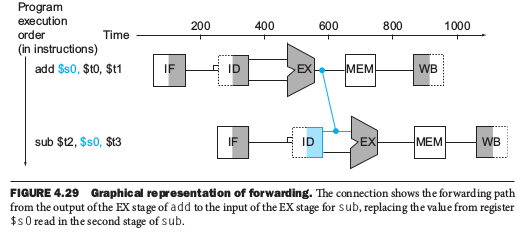
\includegraphics[width=\textwidth]{branch-forwarding}
  \label{fig:branch-forwarding}
  \caption{Esquema de Branch Forwarding}
\end{figure}

Algumas instruções, como o \texttt{LOAD}, apenas disponibilizam o dado em um estágio muito avançado, atrasando o \textit{pipeline} ao ponto de uma instrução seguinte. O \textbf{pipeline interlock} é o \textit{hardware} que detecta tal hazard e insere \textit{bubbles} o suficiente até que o \textit{forwarding} possa ser realizado corretamente e a execução continue.

\begin{figure}
  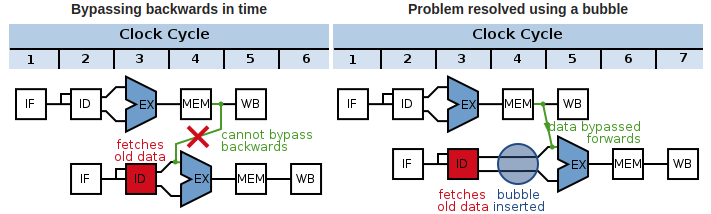
\includegraphics[width=\textwidth]{pipeline-interlock}
  \label{fig:pipeline-interlock}
  \caption{Inserção de \textit{bubbles} para acontecer o \textit{forwarding}}
\end{figure}

O compilador também pode auxiliar, identificando e evitando certos padrões, reeordenando o código de forma a evitar os \textit{stalls}. Chamamos isso de \textbf{pipeline scheduling}, onde o programa é separado em os blocos básicos e as instruções são escalonadas dentro deles.

\textbf{Blocos Básicos:} sequência de instruções onde não há desvios ou I/O. Todas as instruções são executadas se a primeira for.




\subsubsection{Hazard de Controle}
Define-se como \textbf{o atraso resultante da espera de saber se um desvio é tomado}. A instrução de desvio pode mudar o \texttt{PC} (\textit{branch taken}) ou não (\textit{not taken}) e, se tomado, este resultado só será conhecido no estágio \textsc{Mem}. Podemos reduzir combinando a previsão de tomada do desvio e cálculo prévio do novo do \texttt{PC}.

\textsc{Previsão Not Taken}\\
Todos os \textit{branchs} são tratados como \textit{not taken} e o \textit{pipeline} é carregado com as instruções seguintes a ele. O estado da máquina não é alterado até o desvio ser conhecido e se a previsão falhar, as mudanças são desfeitas, o que chamamos de \textbf{back out}.

\textsc{Previsão Taken}\\
Todos os \textit{branchs} são tratados como \textit{not taken} e o \textit{pipeline} é carregado com as instruções a partir do endereço apontado por ele. Não é muito efetiva, já que em várias arquiteturas ainda não se conhece o alvo do desvio.

\textsc{Delayed Branch}\\
Muito usado nos primeiros RISCs. O compilador tenta inserir um conjunto de instruções que sempre será executado após o \textit{branch}, independente do seu resultado. Chamamos este conjunto de \textbf{\textit{branch delay slot}}, o qual estará sempre após a instrução de desvio e normalmente tem tamanho 1. Há três formas de se escalonar:

\begin{itemize}
  \item \textbf{From before:} retira instruções \underline{independentes do desvio e posteriores a ele}, inserindo-as no \textit{slot}. Esta é a melhor opção e deve sempre ser tomada quando possível;

  \item \textbf{From target:} usado quando há maior probabilidade de \underline{desvio \textit{taken}}. Insere no \textit{slots} as instruções presentes no endereço do desvio. Se a previsão falhar, haverá trabalho disperdiçado;

  \item \textbf{From fall through:} usando quando há maior probabilidade de \underline{desvio \textit{not taken}}. Insere no \textit{slot} as instruções logo depois da instrução do desvio.
\end{itemize}

\begin{figure}
  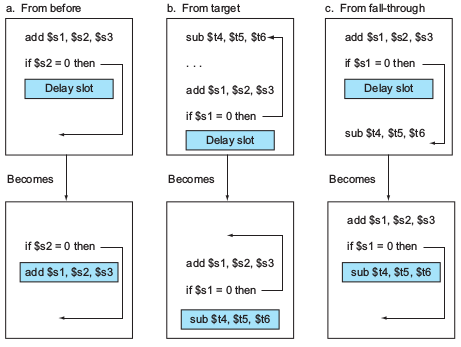
\includegraphics[width=\textwidth]{delayed-branch-scheme}
  \label{fig:delayed-branch-scheme}
  \caption{Escalonamentos do delayed branch}
\end{figure}

Se a previsão é correta, o \textit{delay slot} é executado. Caso contrário, fazemos o \textbf{cancelamento do \textit{branch}}: inserimos um \texttt{NOP} no \textit{delay slot} e executamos. Isso remove restrições extras a serem colocadas no \textit{slot}. Normalmente, os \textit{cancelling branches} são tomados quando há o \textit{not taken}.

Esta técnica possui limitações. Em tempo de compilação, é difícil de prever se vai haver o desvio e o conjunto de instruções podem conter outras depêndencias e \textit{branches} que impedem a previsão.




\section{Barramento}
\textsc{Definição:} meio de transmissão compartilhado que conecta dispositivos. Sua velocidade máxima é limitada pelo seu tamanho e o número de dispositivos conectados a ele.

Barramentos do tipo CPU-Memória são pequenos e de alta velocidade, enquanto os de I/O são maiores, acomodando diversos tipos de dispositivos, seguindo um determinado padrão.

Um barramento é composto por:

\begin{itemize}
  \item \textbf{Linhas de dados:} cada linha transporta 1 bit por vez;

  \item \textbf{Linhas de endereço:} onde o endereço da palavra acessada é colocado

  \item \textbf{Linhas de controle:} controlam o uso das linhas
    \begin{itemize}
      \item Memory write \& memory read
      \item Transfer ACK
      \item Bus request, que pede o controle do barramento
      \item Bus grant, que obtém o controle do barramento
      \item Clock e reset
    \end{itemize}
\end{itemize}

\begin{figure}
  \centering
  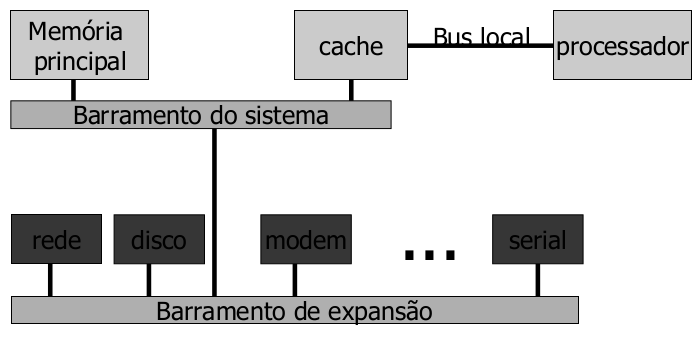
\includegraphics[width=0.8\textwidth]{buses-arch}
  \label{fig:buses-arch}
  \caption{Arquitetura com diferentes barramentos}
\end{figure}

A \textbf{leitura de dados da memória} é feita com o envio de um endereço e sinais de controle indicativo leitura. A memória coloca o dado no barramento e retira - ou \textit{deasserts} - o sinal de espera (\textit{wait}).

A \textbf{escrita dos dados em memória} é feita com a CPU enviando o endereço e do dado ao barramento. A memória retira estes sinais e atualiza o dado. Geralmente, a CPU não espera a confirmação.

Os \textbf{bus masters} são dispositivos que podem iniciar transações no barramento, como a CPU. Sistemas com vários masters necessitam de um esquema de arbitragem para resolução de conflitos, geralmente usando prioridade fixa ou randômica.


\textbf{Split transaction buses} são buses \textit{pipelined} ou \textit{packet-switched}. As transações no barramento são divididas em etapas, de forma a não bloquear o mesmo durante toda a transação. A unidade envolvida participa da arbitragem. As transações possuem \textit{tags}, para serem identificadas.

\underline{Exemplo:} transação de \textit{read} pode ser dividida em \textit{read-request} e \textit{memory-reply}.



\subsection{Síncronos x Assíncronos}
Nos \textbf{barramentos síncronos} uma das linhas de controle é um \textit{clock}. Os protocols para endereço e dados são fixos e baseados neste \textit{clock}. Normalmente são os barramentos CPU-Memória, uma vez que são rápidos e baratos. Devidos as distorções no \textit{clock} (\textit{clock skew}), eles não podem ser longos.

Já \textbf{barramentos assíncronos} usam protocolos de \textit{handshaking} entre o emissor e receptor do dado, provando um \textit{overhead} de sincronização a cada transação. Por isso são mais lentos, mas permitem que mais tipos de dispositivos sejam utilizados, sendo ótimos para gerênciar \textit{buses} de I/O.

	\chapter{Cache e RAM}

\textsc{Definição} \textbf{Princípio de Localidade:} programas tendem a reusar dados e instruções que foram usadas recentemente. Podemos dividir em:

\begin{itemize}
  \item \textbf{Localidade temporal:} itens acessados recentemente têm grande probabilidade de serem acessados novamente;

  \item \textbf{Localidade espacial:} itens cujos endereços estão próximos tendem a ser acessados em tempos próximos.
\end{itemize}

Logo temos a possibilidade de prever instruções que serão utilizadas em um futuro próximo com base em acessos recentes. Isso justifica o uso da \textbf{hierarquia de memória}.


\section{Cache}
\textsc{Definição} Memória rápida e com pouca capacidade de armazenamento. Interposta entre a CPU e a memória principal. A medida de dados é feita em \textbf{WORDS} (palavras), a qual normalmente trocada entre CPU e cache. Definimos:

\textbf{Cache hit:} o dado procurado está em cache

\textbf{Cache miss:} o dado procurado NÃO está em cache

\begin{figure}[ht]
  \centering
  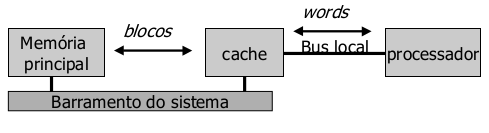
\includegraphics[width=0.8\textwidth]{cache-arch}
  \label{fig:cache-arc}
  \caption{Detalhes de ligação entre cache, processador e memória}
\end{figure}

\subsection{Colocações e Localização de Bloco em Cache}
A cache é bem menor que a memória, logo precisamos de um modo de inserir blocos da memória na cache e indexa-los de forma eficaz. O formato de um endereço do ponto de vista da \textit{cache} segue a Figura \ref{fig:address-cache}. Dentro de um endereço de tamanho $A$, temos:

\begin{figure}[ht]
  \centering
  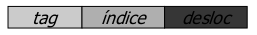
\includegraphics[width=0.6\textwidth]{cache-addr}
  \caption{Estrutura do endereço do dado, do ponto de vista da \textbf{cache}}
  \label{fig:address-cache}
\end{figure}

\begin{itemize}
  \item \textbf{Índice - $I$}: a posição do bloco dentro da cache. No caso do set associative, é o índice do conjunto em que o bloco se encontra.
  \begin{equation}
    I = \lg{\frac{C}{b}}
  \end{equation}

  \item \textbf{Deslocamento - D}: é índice da palavra em que o dado se encontra, em relação ao bloco. Deve ser o número de bits para representar o número de palavras em um bloco;
  \begin{equation}
    D = \lg{w}
  \end{equation}

  \item \textbf{Tag - T}: verificador usado para indicar se há um miss ou um hit na hora do acesso. É sempre o que sobra no endereço depois do índice e deslocamento.
  \begin{equation}
    T = A - (I + D)
  \end{equation}
\end{itemize}

A seguir, iremos definir como esse endereço se estrutura ao longo dos três tipos de colocação do bloco em cache. A Figura \ref{fig:cache-placement} dá um ótimo exemplo de como um mesmo dado é colocado e disponibilizado ao longo dos três métodos. Antes, defina que a cache tem tamanho $C$, com blocos de tamanho $B = w.b$, onde $w$ é o tamanho da palavra e $b$ o número de bytes por palavra. Para sabermos o número total de blocos $N_B$ dentro da cache, usaremos a Equação \ref{eq:cache-blocks}.

\begin{equation}
N_B = \frac{C}{b}
\label{eq:cache-blocks}
\end{equation}

\begin{figure}[ht]
  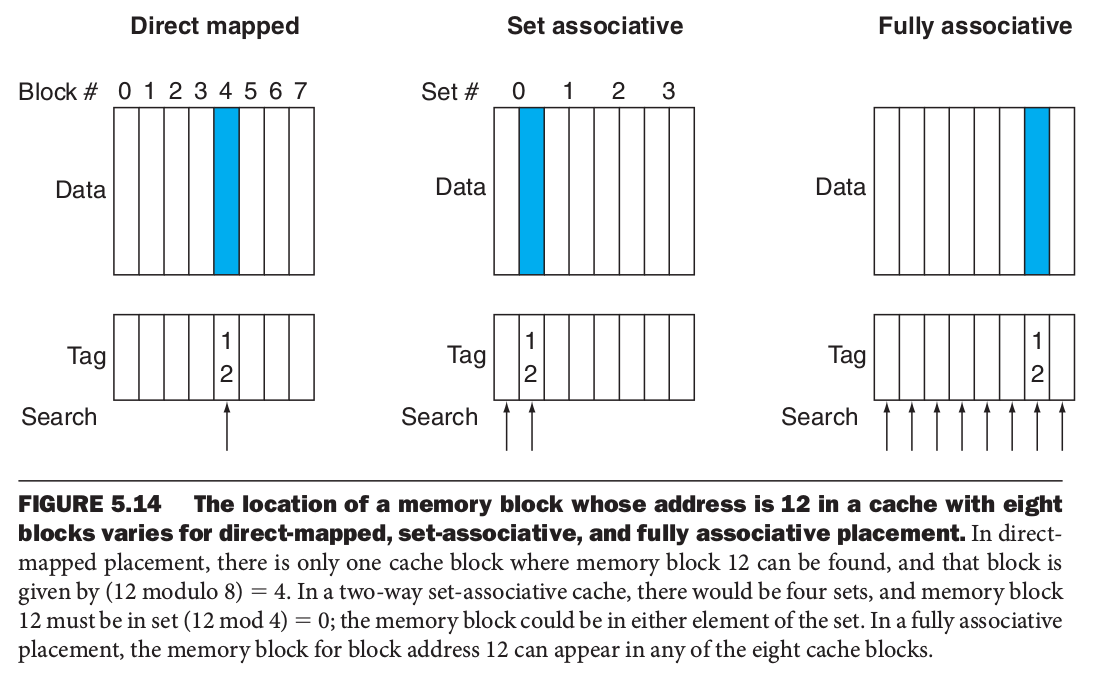
\includegraphics[width=\textwidth]{cache-placement}
  \caption{Diferentes abordagens para colocação de cache. Desenho retirado do Patterson}
  \label{fig:cache-placement}
\end{figure}



\textsc{Mapeamento Direto}\\
O bloco só pode ser posto em um lugar na \textit{cache}, ou seja, o bloco da memória ocupa uma única linha da \textit{cache}. Para achar a linha fazemos:

\begin{equation}
  i = B_M \text{ mod } N_B
\end{equation}

onde $i$ é o número da linha e $B_M$ o número do bloco da memória principal.



\textsc{Set Associative}\\
Aqui o bloco pode ser colocado em um conjunto de blocos. Ao ser acessado novamente, o controlador tem que procurar o bloco dentro deste conjunto. Dentro do conjunto, o bloco pode ser colocado em qualquer posição (varia por algoritmo).

Quando temos $n$ blocos em cada conjunto, a colocação em \textit{cache} é chamada $mn$-way \textit{set associative}. Observe que 1-way set associative equivale ao mapeamento direto. Dado isso, o índice diminui, pois há um número menor de índices na cache e o cálculo do seu tamanho no endereço se dá por:

\begin{equation}
  I = \lg{\frac{C}{n.b}}
\end{equation}



\textsc{Fully Associative}\\
Aqui o bloco pode ser posto em qualquer lugar da \textit{cache}, ou seja, o conjunto de blocos é a cache inteira. Logo o bloco pode ser colocado em qualquer lugar da cache, o que leva a diminuição de misses, pois os blocos não tem uma posição fixa. Entretanto, há um overhead: para obter o bloco, devemos procurá-lo pela cache inteira.

Como não há índice de blocos e conjunto, \textbf{o tamanho do índice no endereço é 0} e só temos o deslocamento e a tag.




\subsection{Substituição de Blocos em \textit{Cache}}
Quando há um \textit{cache miss}, o controlador da cache deve selecionar um bloco para ser substituído. Em \textit{caches} de mapeamento direto, não há escolha, pois somente um bloco pode ser substituído.

Já em esquemas associativos há duas maneiras:
\begin{itemize}
  \item \textbf{Random:} visando uniformidade, os blocos são selecionados aleatoriamente;

  \item \textbf{LRU:} substitui blocos menos recentemente utilizados. Esta tem técnica tem custo alto e geralmente são usadas aproximações.
\end{itemize}


\subsection{Leitura de Blocos em \textit{Cache}}
A leitura e comparação de \textit{tag} pode ser feita simultaneamente. Por isso, a leitura já é feita quando o endereço está disponível.

Se temos um \textit{read hit}, o dado é repassado a CPU imediatamente. Se temos um \textit{miss}, a leitura prévia é ignorada e o bloco é carregado da memória principal. O diagrama da Figura \ref{fig:reading-cache} mostra as transições.

\begin{figure}[ht]
  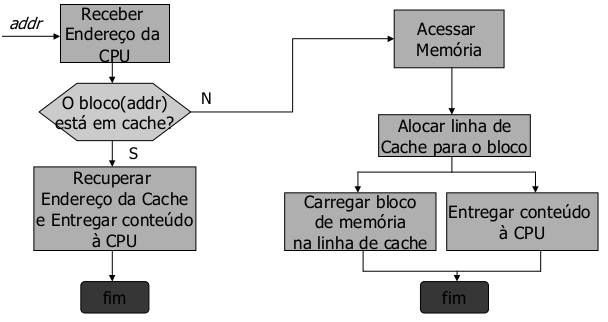
\includegraphics[width=\textwidth]{cache-read}
  \caption{Fluxograma de decisão de leitura da cache}
  \label{fig:reading-cache}
\end{figure}

\subsection{Escrita de Blocos em \textit{Cache}}
Bloco só podem ser alterados/escritos após a confirmação da \textit{tag}, o que torna a operação mais lenta. Além disso, os processadores informam o número de bytes exatos a serem escritos, limitando a operação a essas posições. Na leitura, o acesso à dados a mais não trás problemas.

Temos duas políticas de escrita:
\begin{itemize}
  \item \textbf{Write-through:} dado escrito tanto no bloco em \textit{cache} como na memória. São políticas mais simples e os \textit{read misses} nunca ocasionam escritas para a memória, já que essa política garantem sempre os dados válidos na memória a cada escrita;

  \item \textbf{Write-back:} dado é escrito somente em \textit{cache}. Apenas quando há substituição que o bloco modificado é escrito em memória. Acabam por ser mais rápidas, pois ocorrem só na velocidade de \textit{cache} e usam menos largura de banda já que envia nada a memória.
\end{itemize}

\textsc{Definição} \textbf{Dirty bits:} indicam se o bloco foi modificação enquanto estava em \textit{cache} (\textit{dirty}) ou não (\textit{clean}), sendo que estes últimos não são escritos em memória na substituição.

\textsc{Definição} \textbf{Write Stalls:} ocorrem quando a CPU tem que esperar que o dado seja escrito em memória. Para reduzir este tempo, são usada \textbf{write-buffers}, onde a CPU escreve o dado e continua suas tarefas. O dado então é enviado de maneira assíncrona para a memória.

Em um \textbf{write miss}, o dado antigo não é mais necessário e logo temos duas abordagens para tal:
\begin{itemize}
  \item \textbf{Write allocate:} o bloco é carregado em \textit{cache} no momento do \textit{write miss} e logo depois o \textit{write hit} ocorre;

  \item \textbf{No-write allocate:} o bloco é modificado em memória e não é carregado em \textit{cache}.
\end{itemize}

Políticas \textit{write-back} tendem a usar o primeiro e \textit{write-through} o segundo.

\subsection{Medidas de Desempenho}
Calculamos o tempo média de acesso à memória:
\begin{equation}
  A = T + M * P
\end{equation}

onde $A$ pode ser medido em frações de segundo ou ciclos de clock e:

\begin{itemize}
  \item \textbf{Hit time - $T$:} tempo gasto em um \textit{hit} em cache;
  \item \textbf{Miss rate - $M$:} taxa de misses na cache;
  \item \textbf{Miss penalty - $P$:} penalidade associada a cada miss.
\end{itemize}






\section{Melhoria de Desempenho de Cache}
As caches foram introduzidas para reduzir o gap entre os tempos de aceso à memória principal e a velocidade do processador. O ideal de um projeto de cache seria obter hits rápidos e poucos misses. Logo, temos que melhorar o desempenho dessas caches.

Em se tratando de \textbf{tipos de cache misses}, tempos três tipos, onde eles são relacionados no gráfico da Figura \ref{fig:misses-by-access}:

\begin{itemize}
  \item \textbf{Compulsórios:} no primeiro acesso ao bloco, o mesmo não estará na cache e logo deverá ser trazido para a memória. Também chamados de \textit{cold misses} ou \textit{reference misses};

  \item \textbf{Capacidade:} ocorrem quando um bloco escolhido para substituição é acessado novamente;

  \item \textbf{Conflito:} ocorrem em caches com mapeamento direto ou associativas, se muitos dos blocos referenciados são mapeados para o mesmo conjunto. Também chamados de \textit{collision misses} ou \textit{interference misses}.
\end{itemize}

\begin{figure}[ht]
  \centering
  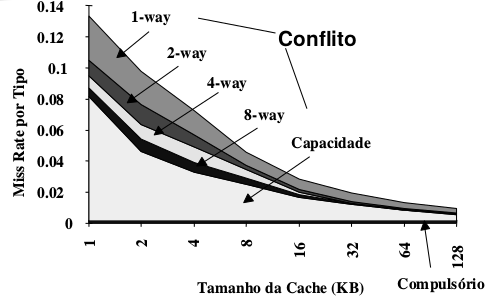
\includegraphics[width=0.8\textwidth]{misses-by-access}
  \caption{Taxas de \textit{misses} por tipo de acesso em um SPEC92, por Patterson}
  \label{fig:misses-by-access}
\end{figure}

\subsection{Reduzindo Cache Misses}

\subsubsection{Aumentar o Tamanho do Bloco}
Quanto maior o tamanho do bloco, menor o número de misses compulsórios, baseando-se no princípio de localidade temporal. Porém, blocos grandes fazem aumentar o número de misses de conflito e capacidade e aumentam a penalidade do miss.
% TODO: não seria espacial??

A escolha do tamanho do bloco leva em conta a latência (tempo de acesso) à memória e a largura de banda à mesma. Em geral, se a largura de banda e a latência são grandes, blocos grandes são escolhidos.

\begin{figure}[ht]
  \centering
  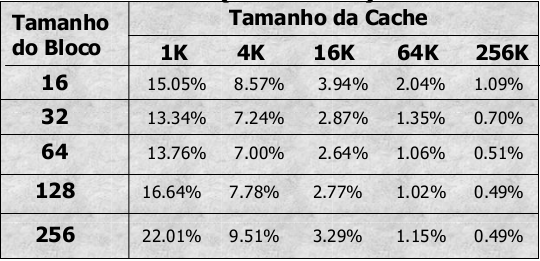
\includegraphics[width=0.8\textwidth]{miss-rate}
  \label{fig:miss-rate}
  \caption{Proporção de \textit{miss rate} ao balancear tamanho de bloco e tamanho de cache}
\end{figure}


\subsubsection{Aumentar a Associatividade}
A justificativa desta técnica é que com maior associatividade, há mais blocos que potencialmente podem ser escolhidos para substituição, possibilitando o uso de algoritmos mais elaborados.

Para utilizar essa técnica, deve-se observar duas regras gerais, obtidas empiricamente:
\begin{itemize}
  \item Uma cache 8-way set associative reduz a taxa de misses tanto quanto uma cache totalmente associativa.

  \item Uma cache de mapeamento direto de tamanho $N$ apresenta aproximadamente o mesmo miss rate que uma cache 2-way associativa de tamanho $\frac{N}{2}$.
\end{itemize}

Logo, devemos ter em mente que, ao aumentar a associatividade, o projeto da cache fica mais complexo e, portanto, o tempo de hit aumenta. Logo, tem de ser pesar as duas grandezas, pois é capaz do tempo médio aumentar.


\subsubsection{Caches Vítimas}
A cache vítima é uma pequena cache totalmente associativa que é adicionada entre a cache e o nível inferior de memória imediatamente inferior. A cache vítima contém somente blocos que foram substituídos da cache por causa de um miss.

Na ocorrência de um misss, verifica-se se o bloco encontra-se na cache vítima. Se sim, o bloco vítima substitui um bloco da cache. Alguns estuso mostram que caches vítimas de poucos bloco (4 em geral) conseguem reduzir o número de misses de conflito de caches pequenas de mapeamento direto.



\subsubsection{Caches Pseudo-Associativas}
Também chamadas de associativas por coluna, essas caches tentam obter a taxa de misses da cache associativa e o tempo de hit da cache de mapeamento direto.

No caso de hit, o acesso a esta cache funciona como o de um mapeamento direto. Em caso de miss, o pseudo-set é obtido pela inversão dos bits mais significativos do índice e a entrada da cache obtida desta maneira é verificada.

Elas possuem um tempo de hit rápido e um tempo de hit lento. Como tal tempo é variável, isso pode complicar o projeto do pipeline. Logo, ela é mais adequada em caches de segundo nível.



\subsubsection{Pré-carga por Hardware de Instrução e Dados}
Intuitivamente, a taxa de misses pode se reduzida se trouxermos os dados e instruções para cache antes dos mesmos terem sido referenciados. É uma ténica comum trazer dois blocos a cada miss: o bloco referenciado e o próximo (localidade espacial). O bloco referenciado é colocado na cache o próximo em um \textit{stream buffer}.



\subsubsection{Pré-carga com Auxílio do Compilador}
Aqui, o compilador insere instruções de pré-carga no código do programa. Em geral, garantimos que o dado ou instrução pré-carregados não causarão excessões de memória virtual (reais ou de proteção). Por esta razão, as pré-cargas mais efetivas são as que não causam alteração no programa (\textit{non-binding prefetching}).

A pré-carga só faz sentido se o processador puder continuar a operação enquanto o dado a ser pré-carregado não chega. Note que as caches devem ser capazes de tratar diversas requisições sem se bloquear (\textit{lockup-free caches}).

A execução de instruções de pré-carga adiciona um overhead à execução, logo é necessário certificar que ele não irá aumentar o tempo geral.



\subsubsection{Otimizações do Compilador}
Técnicas em código, sem usar hardware adicional. Podem ser usadas técnicas de profiling para rearrumar o código, reduzindo misses das instruções.

\textsc{Merging de Arrays}\\
Ao referenciar \textit{arrays} com o mesmo índice no mesmo \textit{loop}, acabamos por gerar misses de conflito, já que as posições dos arrays podem estar em blocos diferentes.

\begin{figure*}[ht]
  \begin{subfigure}[t]{.5\textwidth}
    \centering
    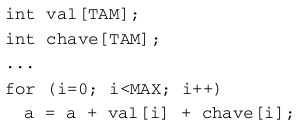
\includegraphics[width=\textwidth]{array-merge-1}
    \caption{\textbf{Código original:} dois \textit{arrays} logicamente conectados, sendo percorridos. Aqui a cada acesso distindo à \texttt{chave{[i]}} e \texttt{valor{[i]}}, podemos ter troca de bloco no cache}
  \end{subfigure}
  ~
  \begin{subfigure}[t]{.5\textwidth}
    \centering
    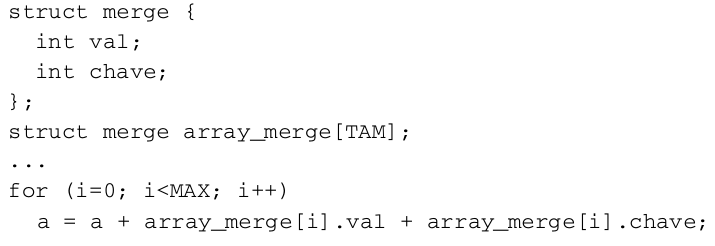
\includegraphics[width=\textwidth]{array-merge-2}
    \caption{\textbf{Código arrumado:} Agora os dados estão sob uma mesma \textit{struct}, logo estão adjacentes na memória. Ganho na localidade espacial quando o bloco for carregado.}
  \end{subfigure}

  \caption{Exemplo de reestruturação de código para \textit{array merge}}
  \label{figs:array-merge}
\end{figure*}




\textsc{Troca de Loops}\\
Loops aninhados que não acessam dados de maneira sequencial podem acabar por acessar bloco diferentes a cada alternância entre as posições. Acesso à matrizes é um bom exemplo. O compilador pode alterar o código de maneira que o acesso seja sequencial.

\begin{figure*}[ht]
  \begin{subfigure}[t]{.5\textwidth}
    \centering
    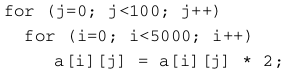
\includegraphics[width=\textwidth]{loop-exchange-1}
    \caption{\textbf{Código original:} exemplo de acesso não sequencial, onde se itera por linha na matriz}
  \end{subfigure}
  ~
  \begin{subfigure}[t]{.5\textwidth}
    \centering
    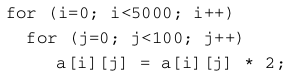
\includegraphics[width=\textwidth]{loop-exchange-2}
    \caption{\textbf{Código arrumado:} agora iteramos por coluna, aproveitando a localidade espacial}
  \end{subfigure}

  \caption{Exemplo de reestruturação de código para troca de \textit{loops}}
  \label{figs:loop-exchange}
\end{figure*}



\textsc{Junção de Loops}\\
O acesso a matrizes com os mesmo loops porém fazendo cálculos diferentes. Logo, podemos tirar proveito da localidade temporal, fazendo que os dados sejam acessados diversas vezes enquanto então em cache.

\begin{figure*}[ht]
  \begin{subfigure}[t]{.5\textwidth}
    \centering
    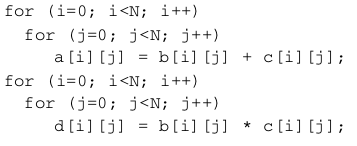
\includegraphics[width=\textwidth]{loop-merge-1}
    \caption{\textbf{Código original:} dois loops iterando sobre a mesma matriz, mas fazendo operações diferentes}
  \end{subfigure}
  ~
  \begin{subfigure}[t]{.5\textwidth}
    \centering
    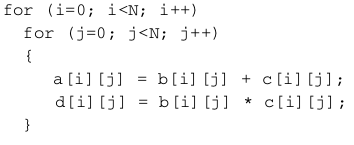
\includegraphics[width=\textwidth]{loop-merge-2}
    \caption{\textbf{Código arrumado:} junção dos dois loops originais em um só. Tiramos proveito da localidade temporal para os dois loops, dado que os dados já estarão em cache}
  \end{subfigure}

  \caption{Exemplo de reestruturação de código para junção de \textit{loops}}
  \label{figs:loop-merge}
\end{figure*}





\textsc{Blocagem}\\
As vezes, quando diversas matrizes são acessas sendo umas por linhas e outras por colunas, podemos realizar uma otimização mais complexa. Operamos em submatrizes (ou blocos), ao invś de se operar sobre a matriz inteira.

\begin{figure*}[ht]
  \begin{subfigure}[t]{.5\textwidth}
    \centering
    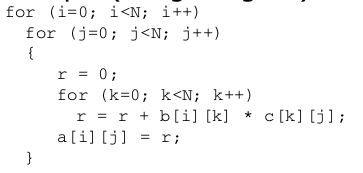
\includegraphics[width=\textwidth]{blocking-1}
    \caption{\textbf{Código original:} \texttt{a} e \texttt{b} percorrem por linha, enquanto \texttt{c} percorre por coluna. Percorremos a matriz inteira sequencialmente.}
  \end{subfigure}
  ~
  \begin{subfigure}[t]{.5\textwidth}
    \centering
    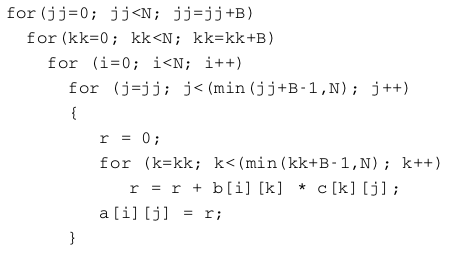
\includegraphics[width=\textwidth]{blocking-2}
    \caption{\textbf{Código arrumado:} criação de submatrizes e percorrimento dessas}
  \end{subfigure}

  \caption{Exemplo de reestruturação de código com blocagem}
  \label{figs:blocking}
\end{figure*}




\subsection{Reduzindo Penalidade do Miss}

\subsubsection{Priorizar Misses de Leitura}
Para acelerar a conclusão da execução de instruções, geralmente \textit{write buffers} são adicionados ao hardware. Logo, quando o store termina, geralmente o dado se encontra neste buffer e não no bloco de cache associado.

Esta decisão pode fazer com que dependendo da ordem de acesso aos dados, valores antigos sejam lidos.

\underline{Exemplo:}

\texttt{1. LOAD 512, r3}\\
\texttt{2. LOAD r1, 1024}\\
\texttt{3. LOAD r2, 512} \\

Caso os endereços 512 e 2014 estejam mapeados no mesmo índice de cache e a escrita de (1) demorar a se completar, a instrução 3 pode ler o valor antigo da memória, havendo um hazard RAW de dados.

A maneira mais simples de evitar que este problema aconteça, consiste em fazer com que o read miss espere até que o \textit{write buffer} esteja vazio. Mas isso aumenta a penalidade do read miss.

Para priorizar misses de leitura, o hardware de muitos processadores verificam o contéudo do \textit{write buffer} e, caso não haja conflito, deixa o read miss continuar.



\subsubsection{Utilizar Sub-blocos}
Consiste em dividir cada bloco da cache em sub-blocos e adicionar um bit de validade a cada sub-bloco. O tag continua associado ao bloco.

Em um read miss, somente um sub-bloco é lido da memória e assim temos a redução da penalidade (menos dados).

\begin{figure}[ht]
  \centering
  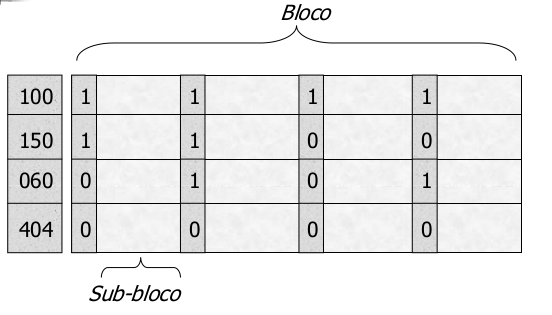
\includegraphics[width=0.8\textwidth]{sub-blocks}
  \label{fig:sub-blocks}
  \caption{Esquema de representação de sub-blocos}
\end{figure}



\subsubsection{Early Restart e Palavra Crítica Primeiro}
Estas técnias não esperam que o bloco inteiro seja colocado em cache, deixando a CPU continuar logo que a palavra desejada esiver carregada.

\begin{itemize}
  \item \textbf{Early restart:} carrega as palavras na ordem sequencial e, logo que a palavra desejada tiver sido carregada, a CPU continuaa a execução.

  \item \textbf{Palavra crítica primeiro:} solicita a palavra que causou o miss primeiro e permite que a CPU continue a execução logo que a mesma chegar
\end{itemize}



\subsubsection{Lockup-free Caches}
Também chamada de \textit{non-blocking cache}, ela é capaz de fornecer dados que estãao na cache mesmo durante um cache miss (\textit{hit under miss}). As mais complexas permitem o tratamento simultâneo de vários misses (\textit{miss under miss}), se a memória for capaz de tratar diversos misses.

O projeto dessas caches é bem complexo, já que lida com diversos acessos incompletos.



\subsubsection{Caches de Segundo Nível}
Como a diferença de desempenho entre RAM e CPU é grande, a inclusão de uma cache mais lentar e de maior capacidade entre a cache tradicional e a memória é interessante. Para serem efetivas, as caches de segundo nível (L2) devem ser bem maiores que a de primeiro nível (L1).

Geralmente, a propriedade de inclusão multinível é observada porém, caso se opte por tamanhos de blocos distintos, o projeto da hierarquia de memória fica complexo.






\subsection{Reduzindo Tempo de Hit}
Esta técnica é interessante uma vez que limita a taxa de clock do processador.


\subsubsection{Caches Simples e Pequenas}
% TODO: ver se está faltando




\subsubsection{Virtual Caches}
Geralmente, a CPU lida com endereços virtuais que devem ser convertidos para endereços físicos e as caches tradicionais utilizam endereços físicos. As caches virtuais utilizam endereços virtuais, não fazendo a tradução de endereços em um cache hit.

No entanto, a cada troca de contexto, a cache deve ser esvaziada (\textit{flushed}), pois cada processo possui seu próprio espaço de endereçamento virtual.



\subsubsection{Pipelining de Escritas}
O pipelining de escritas ocorre entre escritas distintas. Para que o dado seja escrito, primeiramente deve ser feta uma comparação com a tag e depois a escrita é feita no bloco correto. A comparação com a tag é eita no estágio 1 e a escrita no estágio 2.








\section{Memória RAM}
\textsc{Definição} memória semicondutora volátil, onde há a necessidade de um fornecimento constante de energia para manter os valores.

\subsection{DRAM}
Composta por células que armazenam dados, onde um transistor é utilizado para armazenar um bit. É organizada como uma matriz retangular, endereçada por linhas e colunas.

O endereço é dividido em duas metades: \textit{row access strobe} (RAS) e \textit{column access strobe} (CAS). O protocolo de acesso à essa memória é assíncrono. A Figura \ref{fig:dram} mostra o esquema.

\begin{figure}[ht]
  \centering
  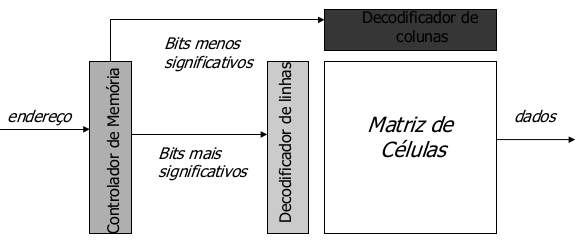
\includegraphics[width=.75\textwidth]{dram}
  \caption{Esquema de acesso à memória DRAM}
  \label{fig:dram}
\end{figure}

As leituras podem danificar o dado contido na célula. Por isso, as DRAMs necessitam de refreshes periódicos para mantê-los. Todos os bits de uma linha podem ser atualizados pela leitura desta linha. Quando há o \textit{refresh}, a memória fica indisponível, um \textit{overhead} que explica o porquê ela é usada mais em memóriais principais.

Para melhorar o desempenho dessas memórias, foca-se em aumentar sua largura de banda. Temos três frentes.

\textsc{Aumento de Tamanho da Palavra}\\
Aumentamos a largura de banda do barramento e logo, transferimos mais dados. Como o acesso da CPU ainda é de uma palavra, é necessário que haja um multiplexador entre a CPU e a \textit{cache}.

\underline{Exemplo:} o Alpha AXP usa barramentos de 256 bits para transferências entre memória RAM e \textit{cache} L2.


\textsc{Memória Entrelaçada}\\
Os chips de memória podem ser organizados em bancos, permitindo que diversas palavras sejam lidas e escritas simultaneamente. Um único controlador de memória é utilizado para isso.

Uma boa função de mapeamento dos endereços para os bancos é crucial para o bom desempenho desta estratégia. A função de módulo normalmente é utilizada,o que favorece acessos sequenciais.

\begin{figure}[ht]
  \centering
  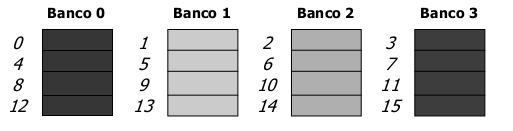
\includegraphics[width=.6\textwidth]{4way-ram}
  \caption{Memória entrelaçada 4-way}
  \label{fig:fourway-ram}
\end{figure}

\textsc{Bancos Independentes de Memória}\\
Aqui existem múltiplos controladores de memória, que permitem que os bancos operem de maneira independente. Cada banco necessita de linhas de endereço separadas e, frequentemente, de barramentos separados.

\subsection{Variações da DRAM}

\textsc{SDRAM}\\
Utiliza um protocol síncrono para troca de dados com o processador, utilizando um relógio externo. O processador informa o endereço e o dado à SDRAM, a qual responde após um número fixo de ciclos de clock. Durante este período, o processador está liberado para outras tarefas.

\textsc{Rambus DRAM}\\
Utiliza um barramento de alta velocidade para trocas entre CPU e memória. Este barramento possui 18 linhas de dados, onde 16 são para o endereço e 2 para paridade. Possui sinais de clock para fazer transações síncronas no barramento.

\textsc{Static DRAM}\\
Utiliza de 4 a 6 transistores por bit, onde os valores binários são armazenados utilizando configurações de flip-flops. o SRAM não necessita de refreshes periódicos, mas ainda precisa de um fornecimento constante de energia.

SRAMs são mais rápidas, mais caras e menos densas que as DRAMs e são muito utilizadas em memórias \textit{cache}.

	\chapter{RISC x CISC}

\textsc{Definição} \textbf{Gap Semântico:} diferença entre as operações oferecidas por uma linguagem e as operações oferecidas pela arquitetura.

A cada vez que as linguagens de programação iam se modernizando, o gap semântico ia aumentando. Ele deu origem a diversas ineficiências na execução dos programas, tamanho excessivo de código binário e complexidade do compilador.

Afim de reduzir esses efeitos, foram projetadas arquiteturas contendo grande número de intruções, diversos modos de endereçamento e instruções complexas oriundas das linguagens de alto nível, surgindo assim as máquinas com conjuntos complexos de intruções, as CISC.

\section{CISC}
Com instruções mais complexas, o objetivo era simplificar o compilador e melhorar o desempenho. Como instruções de alto nível já são traduzidas para linguagem de máquina, por haver uma instrução correspondente, a tradução é mais simples. Porém, um conjunto grande e complexo de instruções traz problemas:
\begin{itemize}
  \item O controle do mecanismos do pipeline é complicado;

  \item O compilador deve agora, ao analisar o código, saber quais instruções de alto nível podem ser diretamente mapeadas para as instruções complexas de máquina, o que nem sempre é fácil;

  \item Muitos compiladores acabam por deixar de usar instruções complexas em suas traduções

  \item O tamanho em bits das instruções em CISC acaba sendo maior que as de RISC;

\end{itemize}

Por isso, o código obtidos de arquitetura CISC são geralmente grande, ainda que visem serem pequenos, rápidos e menores que RISC. Os projetistas advogam que, com instruções maiores e mais complexas, o tempo de execução é reduzido. Porém a unidade de controle de máquinas CISC deve ser mais complexa, ocupando mais espaço, acabando por \textbf{aumentar o tempo de execução de uma única instrução}.


\section{RISC}
Em outra corrente, a eliminação do gap semântico é proposta com arquiteturas mais simples, as RISC. Aqui as instruções são mais simples, permitindo que uma instrução acabe em um ciclo de clock. É dada ênfase em operações entre registradores.

Essas arquiteturas são justificadas com base em estudos dos anos 80 com linguagens de alto nível, identificando que as operações mais abundantes são atribuições (passagem de dados) e desvios. Observou-se também que as variáveis acessadas eram em geral simples e locais, referenciado em média 0.5 operandos em memória e 1.4 registradores por instrução. Por fim, identificou-se que as procedures tinham chamadas menores que 6 parâmetros, usando menos que 6 variáveis locais. Logo não eram necessárias muitas palavras para ativar procedures.

Com base nisso, era mais interessante prover uma arquitetura que atacasse esses padrões de código mais utilizados, o que combinava mais com RISC, do que com arquiteturas que abarcassem aspectos mais gerais, o que se encaixava em CISC.

Como RISC veio como uma contra-proposta a CISC, diversas definições acabaram sendo atribuídas a RISC. Diz-se que "qualquer computador depois de 1985" é RISC. Porém, existem alguns pontos em comum.

\subsubsection{Grande Conjunto de Registradores}
Um número grande de registradores de propósito geral, com uso de compilador para otimizar seu uso. Como o número de atribuições observadas nos estudos eram grandes, os uso de vários registradores otimizava a execução.

Era necessária definir uma estratégia para manter os operandos mais utilizados em registradores e reduzir os acessos à memória. Daí, temos duas estratégias:
\begin{itemize}
  \item \textbf{Por software:} análise do compilador para tentar alocar registradores às variáveis mais utilizadas durante um certo período;

  \item \textbf{Por hardware:} grande conjunto de registradores, permitindo que mais variáveis sejam postas na CPU.
\end{itemize}

Deste último, nasceu a \textbf{janela de registradores}. O conjunto grande de registradores reduz o acesso à memória, mas o projetista deve organizar o acesso de maneira eficiente.

Como a maioria das referências é a variáveis locais, a abordagem mais comum é armazenar essas variáveis em registradores, separando alguns para as variáveis globais.

Porém, variáveis locais são atreladas ao contexto de sua procedure. Na chamada de uma procedure-filha, as variáveis tem de ser salvas em memória para poderem ser utilizadas posteriormente. Ao terminar, teríamos que carregar as variáveis da procedure-pai novamente juntamente com os valores de retorno da filha.

Para resolver isso, as janelas de registradores, que são vários pequenos conjuntos destes, são utilizadas para cada procedure. Uma chamada a uma procedure-filha faz com que uma janela de registradores diferente seja utilizada ao invés de salvar tudo e memória e trabalhar com um conjunto novo. Com isso, procedures adjacentes podem possuir janelas sobrepostas, para facilitar a passagem de parâmetros. Em dado momento, somente uma janela de registradores é visível e endereçavel.

A janela é dividida em 3 regiões de tamanho fixo:
\begin{itemize}
  \item Registradores de Parâmetros
  \item Registradores Locais
  \item Registradores Temporários
\end{itemize}

\begin{figure}[ht]
  \centering
  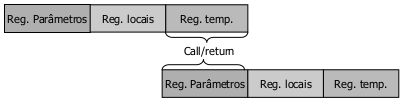
\includegraphics[width=.7\textwidth]{reg-window}
  \label{fig:reg-window}
  \caption{Esquema de uma janela de registradores. Perceba a sobreposição dos temporários e de parâmetros para permitir passagem de valores entre procedures}
\end{figure}

Como só existe um conjunto finito de janelas, somente os dados das procedures mais recentes são mantidos em registradores. Logo os dados de procedures antigas ficam em memória e a organização real do \textit{register file} é uma fila circular de janelas sobrepostas, como mostrado na \ref{fig:window-stack}.

\begin{figure}
  \centering
  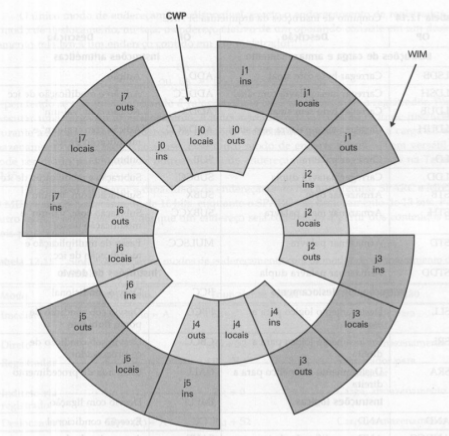
\includegraphics[width=0.66\textwidth]{reg-window-stack}
  \caption{Oito janelas de registradores formando uma pilha circular. Presente em arquiteturas SPARC}
  \label{fig:window-stack}
\end{figure}

\textsc{Variáveis Globais}\\
Se tratando de variáveis globais, inicialmente eram mantidas em memória, sugere-se mantê-las em um conjunto de \textbf{registradores globais} no processador. Estes registradores possuem número fixo e são acessíveis por todas as procedures.

\underline{Exemplo:} podemos dispor os registradores da seguinte forma
\begin{itemize}
  \item Registradores 0-7 contém variáveis globais
  \item Registradores 8-31: referem-se à janela corrente
\end{itemize}

\textsc{Otimizações pelo Compilador}\\
Como em programa escrito em linguagem de alto nível não faz referência a registradores, essa tarefa fica a cargo do compilador, que deve concentrar os acessos nos registradores, reduzindo \texttt{LOAD}s e \texttt{STORE}s.

Em geral, o compilador elege variáveis candidatas para residir em um registrador, chamadas \textbf{\textit{quantity}}, atribuindo-a à um registrador virtual. A idéia é mapear diversos registradores virtuais em um único registrador real, de modo que os virtuais não se sobreponham no tempo. Caso não haja número suficiente de registradores reais em um momento, o compilador recorre à memória.

Para aplicar esta técnica, são aplicados métodos de coloração de grafos. Primeiro o programa é analisado e um grafo de interferências de registradores é construído. O registradores virtuais são os nodos e as interdepêndencias são as arestas. Ao tentar colorir um grafo com $n$ cores, onde $n$ é o número registradores reais, mapeamos os nodos (virtuais) de mesma cor em único registrador real.

\begin{figure}
  \centering
  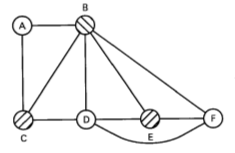
\includegraphics[width=0.6\textwidth]{reg-color-grafo}
  \label{fig:reg-color-grafo}
  \caption{Exemplo de coloração de grafo. Os conjuntos \{$A$, $D$\} e \{$B$, $C$, $E$\} são mapeados em registradores reais. $F$ é mapeado em memória.}
\end{figure}




\subsubsection{Conjunto Pequeno de Instruções}
O conjunto de instruções deve ser projetado de maneira que a grande maioria das \textbf{instruções sejam executada em um ciclo de máquina}, acelerando a execução de programas. A maioria das \textbf{instruções deve ser entre registradores, com operações de \texttt{LOAD} e \texttt{STORE} simples}, o que simplifica as unidades de controle.

A maioria das arquiteturas RISC oferece modos mais simples de endereçamento, geralmente menos que 5. Modos menos comuns de endereçamento, como o indireto e o indexado, podem ser sintetizados via software. Os mais comuns são:
\begin{itemize}
  \item Endereçamento de registradores
  \item ENdereçamento relativo ao PC
  \item Deslocamento
\end{itemize}

Não são usados modos de endereçamento que combinam load/store com operações aritméticas e somente um operando é endereçado a cada instrução. Logo, o formato de instruções são simples, o que permite:
\begin{itemize}
  \item O tamanho da instrução é fixo e alinhado por \textit{word}, com geralmente 4 bytes;

  \item A localização do código da operação é conhecida e de tamanho fixo. Ainda, a decodificação e buscas de operandos pode ser feita simultaneamente.
\end{itemize}

O compilador é uma parte fundamental para a obtenção de um bom código. Além disso, o desenvolvimento de chips RISC são mais rápidos, já que o número de instruções é simples e reduzido.




\subsubsection{Otimizações no pipeline de instruções}
Como arquiteturas RISC possuem instruções simples e regulares, acaba por ser mais fácil otimizar o \textit{hardware} e, consequentemente, no pipeline de instruções.





\section{RISC x CISC}
Observa-se que os projetos de arquitetura CISC vem empregando algumas características de RISC e vice-e-versa.

Como exemplos, as atuais arquiteturas do PowerPC, que é classificada como RISC, empregam implementações de CISC. O Pentium II, apesar de ser classificado como CISC, incorpora diversas características de RISC.

\begin{figure}[ht]
  \centering
  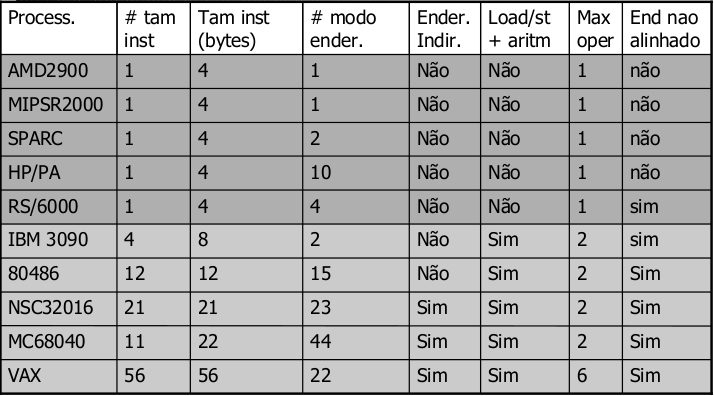
\includegraphics[width=0.75\textwidth]{risc-x-cisc}
  \label{fig:risc-x-cisc}
  \caption{Tabela comparativa de RISC (entradas escuras) X CISC (claras)}
\end{figure}

	\chapter{Instruction Level Parallelism}

\textsc{Definição} o grau no qual instruções de um mesmo programa podem ser avaliadas em paralelo, ou seja, \textbf{a medida de sobreposição potencial entre as instruções}.

\textbf{Note que:} O pipelining é uma das técnicas que explora ILP e é geralmente a base para as demais otimizações propostas.

Um programa pode ser definido como a composição de dois tipos de instruçoes:
\begin{itemize}
  \item \textbf{Atribuições}, da forma $A = B + C$;

  \item \textbf{Branches}, resultando em desvios no fluxo de execução das instruções (condicionais e laços).
\end{itemize}

O código executado entre dois \textit{branches}, i.e. um bloco básico ou \textit{branch path}, é sequencial. Logo, ele é o candidato óbvio para a exploração de paralelismo. No entanto, estudos mostram que tipicamente, o tamanho deste bloco é pequeno, indo de 3 a 0 instruções. Além disso, depêndencias existentes dentro deste bloco acabam por limitar o paralelismo.

Dessa forma, uma técnica efetiva de exploração da ILP deve ser capaz de explorar o paralelismo entre blocos distintos. Os candidatos mais fáceis para tal são as interações de um \textit{loop} - o \textit{loop level parallelism}.

% TODO: por o código
\underline{Exemplo:} aqui, cada iteração do \textit{loop} pode ser executada simultaneamente, apesar de haver a dependência de dados no interior de cada iteração.

\subsubsection{Tarefas do Compilador}
Para manter um pipeline cheio, o paralelismo entre as instruções deve ser explorado de maneira a obter sequências de instruções independentes que possam ser sobrepostas no pipeline. Duas sequências dependentes devem ser separadas por uma distâncias que seja igual à latência do pipeline para a primeira instrução, em ciclos de clock.

A habilidade do compilador de separar instruções está limitada por dois fatores:
\begin{itemize}
  \item A quantidade de ILP presente no programa

  \item As latências das unidades funcionais do pipeline
\end{itemize}

\subsubsection{Quando e Como Explorar o ILP}
Existem diversas técnicas para explorar ILP, onde a maioria necessita que se saiba quando e como a ordem das instruções de um programa pode ser alterada sem que sejam produzidos resultados incorretos.

Deve-se então saber a dependência entre as instruções para se determinar uma maneira de reordená-las sem que as dependências sejam violadas.





\section{Depêndencias}
O grau de dependência entre as instruções determina quanto paralelismo existe em um programa e como o mesmo pode ser explorado. \textbf{Duas instruções serão paralelas quando podem ser executadas simultaneamente em um pipeline, sem a necesidade de atrasos.} Se duas instruções não são paralelas, então elas \textbf{são dependentes} e logo não podem ser reordenadas.

Dependências são propriedades de programas e a presença delas indica o potencial para atrasos no pipeline. Porém, qual atraso e seu impacto é uma propriedade do pipeline.




\subsection{Dependências de Dados}
\textsc{Definição} quando uma instrução depende do resultado de uma instrução específica ou do resultado encadeado de instruções, então temos uma dependência de dados. Também chamada de dependência real.

\begin{figure}[ht]
  \centering
  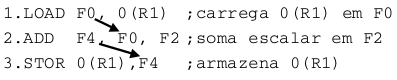
\includegraphics[width=0.6\textwidth]{data-dependency}
  \caption{Aqui, temos uma dependência encadeada: a instrução 3 depende da 2, que depende da 1}
  \label{fig:data-dependency}
\end{figure}

A existência de dependência de dados implica na existência de uma cadeia de \textit{hazards} RAW entre as instruções. Caso as instruções dependentes de dados sejam escalonadas simultaneamente, o pipeline será atrasado.

Uma dependência de dados possui as seguintes características:
\begin{itemize}
  \item Indica a possibilidade de um atraso no pipeline;
  \item Determina em que ordem as operações devem ser executadas;
  \item Determina um limite superior na quantidade de paralelismo que pode ser explorada
\end{itemize}

Pelo fato delas limitarem a ILP, elas devem ser tratadas. Temos duas maneiras:
\begin{itemize}
  \item \textbf{Manter a dependência}, evitando o atraso, o que pode ser feito pelo pipeline ou pelo compilador;

  \item \textbf{Rearrumar o o código} de maneira a eliminar a dependência, feito apenas pelo compilador
\end{itemize}

Um valor de dado pode fluir entre instruções através de registradores ou posições de memória. \textbf{Por um registrador, a detecção de dependência é mais simples, pois os nomes são fixos}. As dependências que ocorrem através de posições de memória possuem um tratamento mais difícil.

\underline{Exemplo:} 100(R2) e 20(R4) podem endereçar a mesma posição de memória, mas é dificil o compilador saber disso. Logo, ele toma o caminho mais conservador que é manter a dependência.





\subsection{Dependências de Nomes}
\textsc{Definição} quando não há valor transferido entre instruções, mas ambas usam o mesmo nome (de registrador ou posição de memória) e pelos menos uma delas altera o valor deste nome, temos uma dependência de nome. Temos dois tipos:

\begin{itemize}
  \item \textbf{Anti-Dependência:} ocorre quando uma instrução lê o valor de um nome e uma outra instrução quer escrever neste mesmo nome. Ou seja, quando \textbf{temos um WAR}. \underline{Exemplo:}

  \begin{center}
    \texttt{ADD R1, R1, R3}\\
    \texttt{LOAD R3, 0(R4)}\\
  \end{center}

  \item \textbf{Dependência de Saída:} ocorre quando duas instruções querem escrever no mesmo nome. Ou seja, quando \textbf{temos um WAW}.
  \underline{Exemplo:}

  \begin{center}
    \texttt{LOAD R1, 0(R2)}\\
    \texttt{ADD R1, R1, 10}\\
  \end{center}
\end{itemize}

Como não há valor sendo transmitido entre instruções, as dependências de nomes são mais fáceis de serem eliminadas se o nome utilizado for alterado, de maneira a remover o conflito. Chamamos isso \textbf{register renaming}. Esta renomeação pode ser feita tanto por \textit{hardware} como por compilador.






\subsection{Dependências de Controle}
\textsc{Definição} quando o ordenamento de uma instrução está atrelado a um \textit{branch}, temos uma dependência de controle.

Toda a instrução, exceto as pertencentes ao primeiro bloco básico, estão atreladas a algum conjunto de \textit{branches} e logo é dependente de controle destes. No caso geral, as dependências de controle devem ser preservadas.

\underline{Exemplo:} vemos abaixo que \texttt{s1} é dependente de \texttt{p1}. Já \texttt{s2} é dependente de \texttt{p2}, mas não de \texttt{p1}\\

\texttt{if (p1) \{ \\  s1\\\}\\if(p2)\{\\  s2\\\}}

Essas dependências geram duas restrições:
\begin{itemize}
  \item Uma instrução que é dependente de controle de um branch não pode ser movida para antes deste branch;

  \item Uma instrução que não é dependente de controle de um branch não pode ser movida para depois do branch, pois caso fosse, sua execução seria então controlada por ele.
\end{itemize}

Em um pipeline básico, as dependências de controle são preservadas por dois motivos:
\begin{itemize}
  \item As instruções são executadas em ordem;

  \item Uma instrução que é dependente de um branch não é executada até que a direção do branch seja conhecida, devido aos hazards de controle.
\end{itemize}

As propriedades a seguir são preservadas pela dependência de controle afim de garantir a correção do programa.



\subsubsection{Comportamento em Face a Exceções}
O reordenamento da execução de das instruções não deve permitir o surgimento de exceções no programa. Por isso, uma postura conservadora é adotada e o reordenamento não é feito, mesmo que não haja dependência de dados.

\begin{figure}[ht]
  \centering
  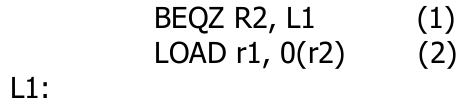
\includegraphics[width=0.6\textwidth]{except-behavior}
  \caption{Se ignoramos a dependência de controle entre 1 e 2, se a instrução 2 é executada antes do branch, podemos levar a um estado de erro, o que não ocorreria se o branch fosse tomado}
  \label{fig:except-behavior}
\end{figure}



\subsubsection{Fluxo de Dados}
\textsc{Definição} o fluxo real de dados entre as instruções que os produzem e as que os consomem.

O branches fazem com que o fluxo de dados seja dinâmico, permitindo que o dado utilizado em determinada instrução possa vir de vários pontos. Logo, o reordenamento não pode afetar este fluxo.

\begin{figure}[ht]
  \centering
  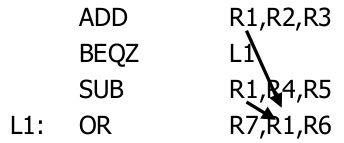
\includegraphics[width=0.6\textwidth]{data-flux}
  \caption{O valor de R1 em 4 vem de 1 se o desvio for tomado e de 3 se não for}
  \label{fig:data-flux}
\end{figure}




\section{Paralelismo a Nível de \textit{Loop}}
A maneira mais simples de se detectar paralelismo é no interior de \textit{loops}. A análise de paralelismo neste nível consiste em se determinar se acesso a dados em iterações posteriores são dependentes de valores de iteração anteriores, i.e., se $i$ depende de $i-1$. Geralmente, esta análise é feita no código fonte, pois a tradução pra a linguagem de máquina cria dependências no registrador de incremento de índice. As Figuras \ref{fig:loop-pal-1}, \ref{fig:loop-pal-2} e \ref{fig:loop-pal-3} refletem bem isso.

\begin{figure*}
  \begin{subfigure}{.45\textwidth}
    \centering
    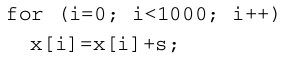
\includegraphics[width=0.9\textwidth]{loop-pal-1}
    \caption{Aqui a dependência ocorre entre os dois usos de \texttt{x{[i]}}, sendo interna a cada iteração. Entre \textit{loops} não há dependencia e eles são paralelos}
    \label{fig:loop-pal-1}
  \end{subfigure}
  ~
  \begin{subfigure}{.45\textwidth}
    \centering
    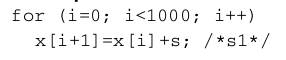
\includegraphics[width=0.9\textwidth]{loop-pal-2}
    \caption{Aqui, \texttt{x{[i+1]}} e \texttt{x{[i]}} dependem, criando dependência entre os laços, obrigando-os a serem executados em ordem. Chamamos esse tipo de \textbf{loop-carried dependencie}}
    \label{fig:loop-pal-2}
  \end{subfigure}
  ~
  \begin{subfigure}{\textwidth}
    \centering
    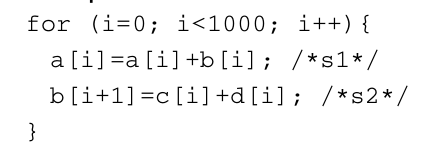
\includegraphics[width=0.5\textwidth]{loop-pal-3}
    \caption{Aqui a dependência é entre \texttt{s1} e \texttt{s2}, pelo fato de \texttt{b{[i]}} depender de \texttt{b{[i+1]}}. Mas note que \texttt{s2} não depende de \texttt{s1}}
    \label{fig:loop-pal-3}
  \end{subfigure}

  \caption{Avaliações de paralelismo a nível de \textit{loop}}
\end{figure*}

Um loop é paralelo se puder ser escrito de maneira que não haja dependência circular entre as dependências \textit{loop-carried}. Note no exemplo da Figura \ref{fig:loop-pal-2} que a dependência é circular, pois \texttt{s1} depende dela própria.

No exemplo da Figura \ref{fig:loop-pal-3}, não há dependência circular, pois \texttt{s2} não depende de \texttt{s1} (mas \texttt{s1} depende de \texttt{s2}). Logo, podemos reescrevê-lo afim de se tornar paralelo. A Figura \ref{fig:loop-pal-fix} mostra o conserto.

\begin{figure}[ht]
  \centering
  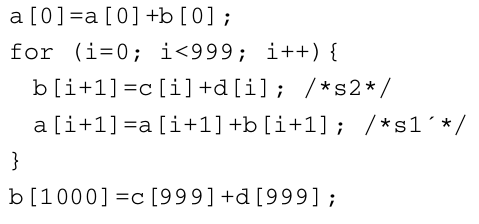
\includegraphics[width=0.6\textwidth]{loop-pal-fix}
  \caption{Agora o loop pode ser paralelo. Semelhante ao exemplo na Figura \ref{fig:loop-pal-1}}
  \label{fig:loop-pal-fix}
\end{figure}






\section{Semântica e Notações de Desvios}
Em desvios condicionais, se a condição for verdadeira, o controle é transferido para a instrução destino do branch - a \textit{branch target address} - e neste caso é dito \textbf{tomado (\textit{taken - T})}. Se a condição é falsa, a execução continua com a instrução imediatamente posterior ao \textit{branch} e o desvio é dito \textbf{não tomado (\textit{not taken - NT})}.

O desvio pode ser \textit{backwards}, indo para trás ou \textit{forward}, indo para frente.



\subsection{Previsões}
Os sinais dos desvios são geralmente preditos por esquemas de previsão de desvio e medimos sua acurácia: \textit{branch prevision accuracy}, ou BPA. O caminho predito é o \textit{predicted path} e o caminho cuja previsão diz que não será tomado é o \textit{not predicted path}.

\textsc{Definição} \textbf{Janela de execução do processador:} parte do código que está em processo de execução na CPU

Um desvio é geralmente previsto depois que entra na janela de execução. Após a previsão, o desvio fica \textbf{pendente}. Quando a condição do desvio é efetivamente avaliada, o branch é dito \textbf{resolvido}.

\textsc{Definição} \textbf{Código estático:} código na ordem de escrita pelo programador ou compilador.

\textsc{Definição} \textbf{Código dinâmico:} diferentes instâncias de instruções estáticas, que surgem durante a execução, ordenadas pelo tempo no qual foram executadas.







\section{Técnicas de Exploração}

\subsection{\textit{Loop Unrolling}}
\textsc{Definição} aumento do bloco básico entre as iterações de um \textit{loop}.

É uma das técnicas mais simples para explorar ILP e implica em um rearrumação do código, normalmente feita pelo compilador. Aplicamos tal técnica em loops independentes, ou seja, loops paralelos. As Figuras \ref{fig:loop-unrolling-1} e \ref{fig:loop-unrolling-2} explicam bem.

Apesar do \textit{loop unrolling} aumentar o tamanho do código do programa, esta transformação é bastante utilizada pois permite o uso mais eficiente do pipeline.

\begin{figure*}
  \begin{subfigure}[b]{.45\textwidth}
    \centering
    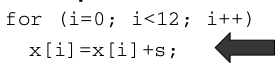
\includegraphics[width=0.9\textwidth]{loop-unrolling-1}
    \caption{Loop paralelo, com bloco básico pequeno}
    \label{fig:loop-unrolling-1}
  \end{subfigure}
  ~
  \begin{subfigure}[b]{.45\textwidth}
    \centering
    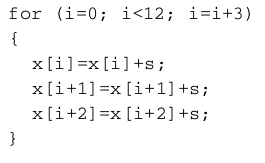
\includegraphics[width=0.9\textwidth]{loop-unrolling-2}
    \caption{Bloco básico estendido e número de iterações menor}
    \label{fig:loop-unrolling-2}
  \end{subfigure}

  \caption{Exemplo de \textit{loop unrolling}}
\end{figure*}


\subsection{Escalonamento Dinâmico}
Permite que o \textit{hardware} reordene a execução das instruções de maneira a reduzir os atrasos no pipeline. Como a reordenação é feita em tempo de execução, o escalonamento é dinâmico. Ele pode ser combinado com o escalonamento estático.

Como \textbf{vantagens}, podemos tratar situações onde as dependências não são conhecidas em tempo de compilação e permite que o código que foi compilada para um tipo de pipeline rode eficientemente em outro tipo. Como \textbf{desvantagens}, temos o aumento da complexidade de \textit{hardware}.

O pipeline básico faz a busca de instruções na ordem do programa. Neste caso, se uma instrução atrasa o pipeline - ou seja, geral um \textit{stall} - nenhuma outra instrução pode prosseguir.

\begin{figure}[ht]
  \centering
  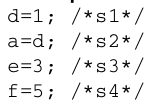
\includegraphics[width=0.4\textwidth]{dynamic-escalo-ex}
  \caption{A instrução \texttt{s2} necessita de \texttt{s1}. Porém, \texttt{s3} e \texttt{s4} são atrasadas, mesmo não dependendo de \texttt{s1} e \texttt{s2}. Podemos eliminar isto se executarmos fora de ordem}
  \label{fig:dynamic-escalo-ex}
\end{figure}

A execução fora de ordem permite que as instruções possam começar sua execução no momento em que seus operando estão disponíveis. Ela também implica que o término das instruções também será fora de ordem, o que pode gerar erros, complicando o tratamento de exceções.

A execução fora de ordem divide o estágio ID em duas partes:
\begin{itemize}
  \item \textbf{Issue:} decodifica as instruções e verifica hazards estruturais

  \item \textbf{Read Operands:} espera até que não haja hazards de dados e lê operandos.
\end{itemize}

A execução de uma instrução se inicia no instante $t$ e termina no instante $v$, onde $v > t$. Em um pipeline com escalonamento dinâmico, todas as instruções entram no estágio \textit{issue} na ordem do programa. Entretanto, no estágio \textit{read operands}, elas podem ser atrasadas ou fazerem um \textit{bypass} das outras instruções - o que é a própria execução fora de ordem.



\subsection{Scoreboarding}
Técnica que permite que as instruções sejam executadas fora de ordem, quando há recursos suficientes e independência de dados. O \textit{scoreboarding} é o elemento principal desta técnica, pois ele controla a execução das instruções e faz a detecção de \textit{hazards}.

Como várias instruções podem estar no estágio EX simultaneamente, o \textit{scoreboarding} \textbf{só é efetivo quando há múltiplas unidades funcionais}.

Toda a instrução que está ou já passou no estágio \textit{issue}, mas não foi terminada, possui um entrada no \textit{scoreboarding}. Ele mantem todas as informaçoes necessárias para detectar as dependências de dados.

O \textit{scoreboarding} determina o instante no qual a instrução pode ler os operando e iniciar a execução. Caso não seja possível, ele monitora toda mudança no \textit{hardware} para determinar quando uma instrução pode ser executada. Por isso, ele controla também quando o resultado pode ser escrito no estágio WB.

Suas etapas são:
\begin{itemize}
  \item \textbf{Issue:} se a unidade funcional destino estiver livre e nenhuma instrução ativa tiver o mesmo registrador destino, o scoreboard faz um issue da instrução. Essas garantias previnem \textit{hazards} WAW.

  \item \textbf{Read Operands:} o scoreboard verifica se os operandos estão disponíveis, ou seja, se nenhuma instrução anterior vai escrever neles. Caso estejam disponíveis, o scoreboard instrui a unidade funcional para a leitura dos mesmos e o início da execução;

  \item \textbf{Execution:} ao receber os operandos, a unidade funcional inicia a execução. Quando o resultado final estiver pronto, o scoreboard é notificado;

  \item \textbf{Write Result:} o scoreboard recebe a notificação e verifica a existência de hazards. Uma instrução $i$ é impedida de escrever seu resultado quando existe uma instrução $j$, precedente a $i$, que não leu os operandos e um dos operandos de $j$ é o resultado de $i$. Ou seja, uma instrução é impedida de escrever seu resultado quando este é o operando de uma outra instrução anterior, que ainda não leu os operandos.
\end{itemize}

A estrutura de dados do \textit{scoreboarding} possui 3 partes:
\begin{itemize}
  \item \textbf{Estado da Instrução:} indica em qual estágio cada instrução está

  \item \textbf{Estado da Unidade Funcional:} possui 9 campos para cada unidade funcional. Eles são: busy, operação, registrador destino (Fi), registradores fonte (Fj,Fk), unidades funcionais que produzem os registradores fonte (Qj,Qk) e flags indicando se os registradores fonte estão prontos (Rj,Rk);

  \item \textbf{Estado do Registrador Resultado:} indica a unidade funcional que escreverá cada registrador
\end{itemize}

O \textit{scoreboarding} apresenta algumas \textbf{deficiências}:
\begin{itemize}
  \item Necessitava de um grande número de barramentos

  \item A escolha das instruções se resumia a um mesmo bloco básico, o que não trás grande paralelismo.
\end{itemize}




\subsection{Tomasulo}
Combina o \textit{scoreboarding} com renomeação de registradores. Possui unidades chamadas \textbf{estações reservas}. Elas servem para armazenar os operando das operações que estão esperando o \textit{issue}, buscando-os logo que os mesmo estiverem disponíveis.

Quando várias escritas são feitas para o mesmo registrador, somente o último é utilizado. Note que os valores anteriores ao último não importam para instruções após a escrita do último. Quando operações são iniciadas, os registradores que contem operando pendentes são renomeados para os nomes das estações reservas, uma vez que elas contém os valores anteriores desse registrador. \textbf{Isso previne \textit{hazards} WAR e WAW}. Como pode haver mais estações reserva do que registradores reais, esta técnica \textbf{pode eliminar mais hazards do que o compilador poderia fazer}.

Cada unidade funcional possui estações reservas próprias, que controlam quando uma instrução pode ser executada naquela unidade, o que garante um controle descentralizado. Os valores dos operandos são obtidos pelas unidades funcionais através de barramentos compartilhados. Isso permite que todas as unidades possam obter o operando simultaneamente. \textit{Loads} e \textit{stores} são tratados como unidades funcionais.

As estações reservas acabam por guardar:
\begin{itemize}
  \item As instruções esperando por execução;
  \item Os operandos destas instruções já calculados ou então a fonte destes;
  \item Informações de controle da execução da instrução.
\end{itemize}

\begin{figure}[ht]
  \centering
  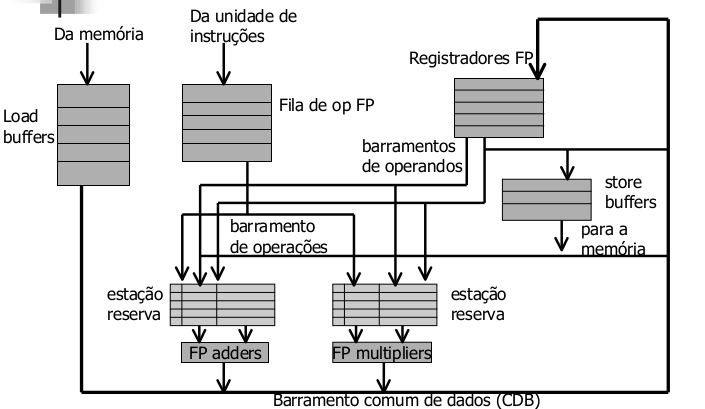
\includegraphics[width=\textwidth]{tomasulo-arch}
  \caption{Arquitetura do Tomasulo}
  \label{fig:tomasulo-arch}
\end{figure}

Temos os seguintes estágios nesta arquitetura:
\begin{itemize}
  \item \textbf{Issue:} retira uma instrução da fila de operações de ponto flutuante. Se há estação reserva livre, inicia a instrução e envia os operandos disponíveis para a estação reserva. Loads e stores podem prosseguir se houver um buffer disponível. Faz também a renomeação dos registradores

  \item \textbf{Execute:} se algum operando não estiver disponível, monitora o CDB. Quando todos os operandos estiverem disponíveis, recupera-os da estação reserva e executa a operação, se não houver hazards RAW;

  \item \textbf{Write Result:} quando o resultado estiver disponível, escreve-o no CDB e também em registradores ou estações reserva que estiverem esperando.
\end{itemize}

A estrutura de dados do Tomasulo possui 6 campos:
\begin{itemize}
  \item \textbf{$Op$:} operação a ser executada

  \item $Q_i$, $Q_j$: estações reserva que produzirão o operando fonte, onde o valor 0 indica que o operando já está disponível ou não é utilizado;

  \item \textbf{$V_i, V_j$:} valor dos operandos $i$ e $j$;

  \item \textbf{Busy/Free}
\end{itemize}

Em termo de \textbf{vantagens} o Tomasulo provê um hardware distribuido para detectar \textit{hazards} RAW e elimina os \textit{hazards} WAW e WAR, através da renomeação de registradores nas estações reservas.

Como \textbf{desvantagens}, temos um necessidade de hardware complexo, o barramento comum dos dados (CDB) pode se tornar um gargalo e não trata o problema dos desvios.






\subsection{Previsão Dinâmica de Desvios}
A frequência dos \textit{branches} torna necessária a utilização de técnicas para reduzir os atrasos potenciais causados por estes desvios, sendo as dependências de controle um grande limitador para a ILP. Nos esquemas de previsão estática de desvios, o comportamento em tempo de execução de cada desvio não é levado em conta. Toda decisão recai sobre o compilador.

A previsão dinâmica de desvios usa o hardware para analisar comportamentos
passados do branch, prevendo seu próximo resultado. A \textbf{efetividade de um esquema de previsão de branches} depende de sua acurácia e do custo de uma previsão correta e de uma previsão incorreta.

Normalmente, os previsores se baseiam em uma tabela de histórico de desvios, chamada \textit{branch history table}, ou \textbf{BHT}. Ela é uma pequena memória, indexada pela porção menos significativa do endereço da instrução de branch, que contem um bit indicando se o desvio foi recentemente tomado ou não.


\subsubsection{Previsão One-bit}
O esquema mais simples de previsão, o qual utiliza a BHT. Prevê que o branch sempre vai ser executado da maneira que foi executado na iteração anterior. Logo, o diagrama de estados segue o mostrado na Figura \ref{fig:one-bit}. Se o \textit{branch} é tomado, a busca instruções continua a partir do endereço do \textit{target} do desvio.

\begin{figure}[ht]
  \centering
  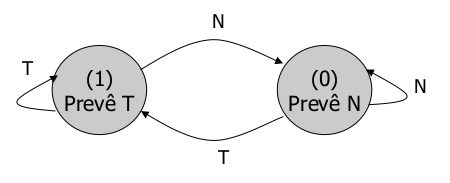
\includegraphics[width=0.75\textwidth]{one-bit}
  \caption{Autômato da Previsão One-Bit}
  \label{fig:one-bit}
\end{figure}

A previsão é uma dica sobre a direção do desvio e a carga de instruções começa a ser prevista. Se a dica estiver errada, o bit de previsão é invertido. Idealmente, deve haver um autômato por \textit{branch} estático. Possui acurácia de 77-79\% e é usado no DEC Alpha 21064, com 2K autômata.

Este esquema tem problemas com loops, onde geralmente ocorrem 2 previsões incorretas.




\subsubsection{Previsão Two-bit}
% TODO: explicar melhor cada autômato

Foi proposto para sanar a deficiênia do esquema de 1 bit, onde agora para haver a alteração de estado, a previsão deve ser incorreta por duas vezes, no mínimo. É possível haver esquemas $n$-bits, onde o de 2-bits faz parte. Um contador é incrementado quando o desvio for tomado e decrementado quando não for. Quando este for maior que $\frac{(2^n - 1)}{2}$, a previsão do desvio é T. Caso contrário, é NT.

A acurária aqui é de de 78-89\% (SPECInt89) e é utilizado no NexGen 586 (2K automata) e no Pentium (256 automata).

\begin{figure*}
  \begin{subfigure}{.5\textwidth}
    \centering
    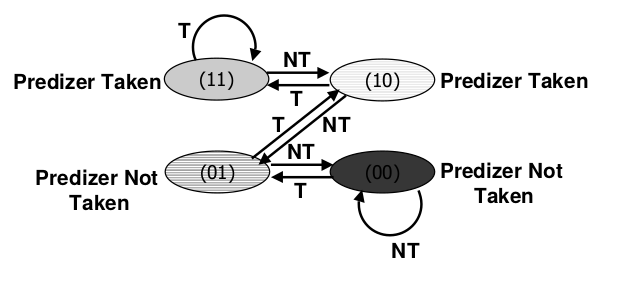
\includegraphics[width=.95\textwidth]{two-bit-sature}
    \caption{Two-Bit Saturada}
    \label{fig:two-bit-sature}
  \end{subfigure}
  ~
  \begin{subfigure}{.5\textwidth}
    \centering
    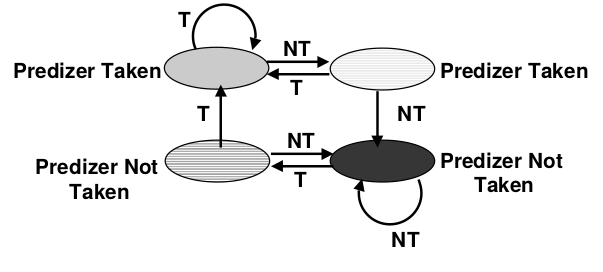
\includegraphics[width=.95\textwidth]{two-bit-patterson}
    \caption{Two-Bit Patterson}
    \label{fig:two-bit-patterson}
  \end{subfigure}
\end{figure*}




\subsubsection{Previsores Correlatos (ou de dois níveis)}
% TODO: melhorar a descrição de funcionamento do funcionamento

Muitas vezes, o comportamento de um branch está relacionado com o comportamento de outro branch. Por isso, os previsores correlatos se baseiam nos últimos branches executados, mesmo que estes não sejam o branch que está sendo previsto. A previsão é feita em dois níveis, com duas estruturas correspondentes:
\begin{itemize}
  \item \textbf{\textit{branch history register} - (BHR):} guarda o história de execução dos desvios. Cada vez que uma instância dinâmica de um branch for resolvida, é feita uma operação de shift a esquerda com seu sinal no BHR. É usado como índice na BPT;

  \item \textbf{\textit{branch pattern table} - (BPT):} armazena um autômato de 2-bits para cada padrão possível no BHR.
\end{itemize}

Esta abordagem possui acurácia de 94.2\% para um BHR de 8 bits e uma BPT de 16 entradas. É usado no NexGen Nx686 e no Pentium Pro (P6).

\begin{figure}[ht]
  \centering
  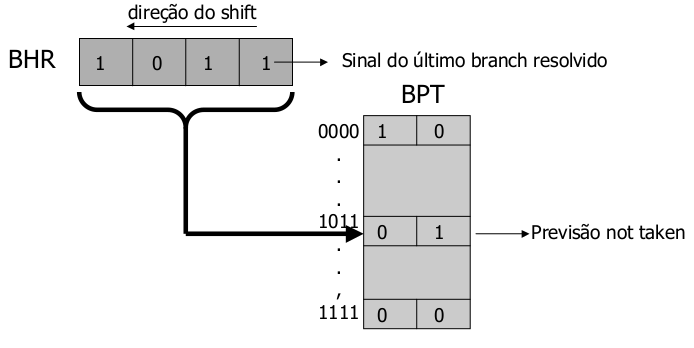
\includegraphics[width=0.85\textwidth]{correlate}
  \caption{Indexação da BHR e BPT na Previsão Correlata}
  \label{fig:correlate}
\end{figure}



\subsubsection{Branch Target Buffer}
Além da previsão da direção, é necessário o endereço da instrução prevista para a execução. Por isso, o \textit{branch target buffer} opera como \textbf{uma cache que guard o endereço previsto da próxima instrução a ser executada após o branch}. Se o PC de uma instrução a ser executada é igual a um PC no BTB, o PC previsto é utilizado como o próximo PC.

Só é necessário guardar os \textit{branches} previstos como \textit{taken}, já que os \textit{branches} não tomados se comportam como as instruções sequenciais.

\begin{figure}[ht]
  \centering
  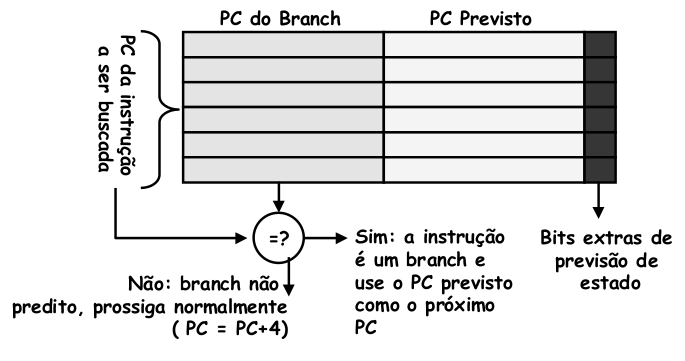
\includegraphics[width=0.85\textwidth]{branch-target-buf}
  \caption{Esquema da previsão dinâmica de buffer, pelo Patterson}
  \label{fig:branch-target-buf}
\end{figure}



\subsection{Execução Especulativa}
A ideia aqui é executar condicionalmente código que está depois de um branch, antes que o branch seja resolvido, o que involve \textbf{a execução do código antes que se tenha certeza de que o mesmo deve ser executado}. É usada em conjunto com a previsão de desvios.

Se a previsão estiver correta, o potencial do ILP é maior do que um caminho do branch. Por isso, o potencial de paralelismo aqui é limitado por duas previsões incorretas (ou \textit{mispredictions}) de direções do branch. A execução especulativa pode ser feita por hardware ou software e temos três tipos, vistos a seguir.



\subsubsection{Single Path}
Neste caso, quando a CPU encontra um branch, o sinal do branch é predito e a
execução prossegue pelo caminho predito. Enquanto o branch não for resolvido, todas as escritas a registradores e memória e todas as operações de I/O devem ser feitas condicionalmente

Estas operações somente serão finalizadas (\textit{committed}) quando todos os branches especulados tiverem sido previstos corretamente. Se houver uma previsão incorreta, as operações não serão finalizas (\textit{squashed}).

O custo em hardware do \textit{single path} é pequeno e cresce linearmente com o número de branches pendentes. Por isso, é o tipo de execução especulativa mais utilizado nos microprocessadores atuais.

\begin{figure}[ht]
  \centering
  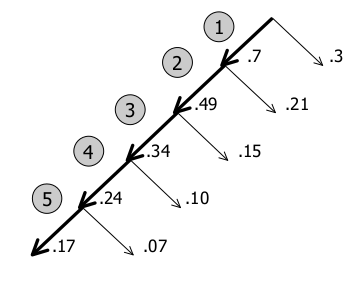
\includegraphics[width=.6\textwidth]{single-path}
  \caption{Exemplo de execução no Simple Path}
  \label{fig:single-path}
\end{figure}




\subsubsection{\textit{Eager Execution}}
Aqui, a execução prossegue pelos dois caminhos do branch, ou seja, não há previsão e sim a execução das duas situações possíveis. Quando um branch é resolvido, todo estado dos caminhos não tomado é descartado.

Sob recursos ilimitados, essa execução oferece o melhor desempenho. Mas com tamanha taxa de descarte e desperdícion, é um algorítmo não realizável.

\begin{figure}[ht]
  \centering
  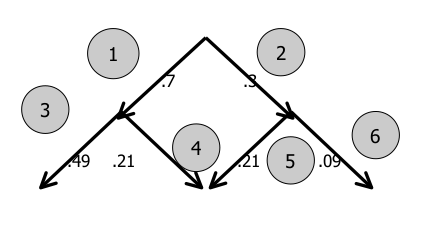
\includegraphics[width=.6\textwidth]{eager-exec}
  \caption{Exemplo de execução no Eager Execution}
  \label{fig:eager-exec}
\end{figure}


\subsubsection{\textit{Disjoint Eager Execution}}
É uma combinação das duas técnicas anteriores, onde os recursos são atribuídos aos branches que tem mais probabilidade de serem executados, considerando todos os branches pendentes. Ou seja, é considerada a probabilidade cumulativa de execução.

Todos os branches são preditos e alguns deles também são executados agressivamente, i. e. os dois caminhos são executados. O custo deste esquema aumenta como uma fração da raiz quadrada do tamanho do caminho principal.

\begin{figure}[ht]
  \centering
  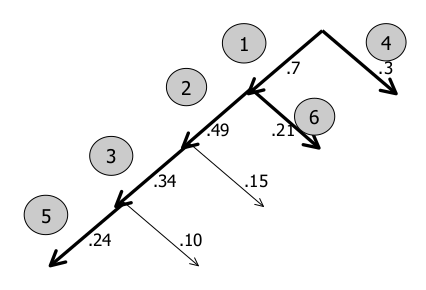
\includegraphics[width=.6\textwidth]{disjoint-eager-exec}
  \caption{Exemplo de execução no Disjoint Eager Execution}
  \label{fig:disjoint-eager-exec}
\end{figure}




\subsection{Arquiteturas Superescalares}
% TODO: indicar se é RISC ou CISC e porque.

\textsc{Definição} Arquiteturas que permitem que diversas instruções sejam iniciadas em um único ciclo de clock e executadas de maneira independente.

Para que isso seja possível, deve-se ser capaz de buscar mais de uma instrução
por ciclo de clock e executar diversas instruções simultaneamente. Entretanto, isso trás uma série de limitações:
\begin{itemize}
  \item \textbf{Dependências}, uma vez que instruções executadas paralelamente podem depender uma da outra;

  \item \textbf{Conflitos estruturais}, onde instruções irão utilizar as mesmas estruturas;

  \item \textbf{Tempos diferentes de execução das instruções}, podendo causar descompassos entre instruções dependentes;

  \item \textbf{Hardware bastante complexo}, dado que a complexidade do hardware depende do número de instruções a serem executadas simultaneamente.
\end{itemize}

\begin{figure}[ht]
  \centering
  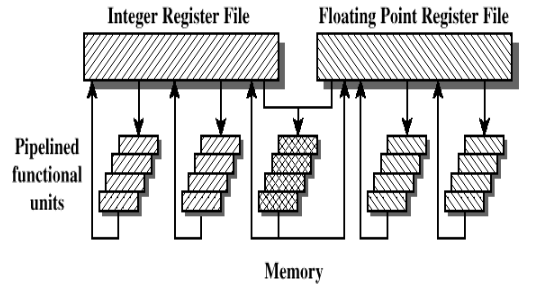
\includegraphics[width=.9\textwidth]{arq-superscalar-org}
  \caption{Organização geral de uma Arquitetura Superescalar}
  \label{fig:arq-superscalar-org}
\end{figure}

\begin{figure}[ht]
  \centering
  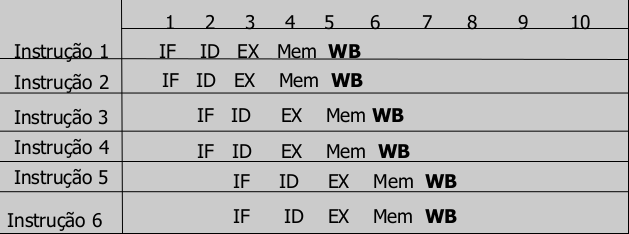
\includegraphics[width=.75\textwidth]{arq-superscalar-exec}
  \caption{Simulação de execução de instruções em Arquitetura Superescalar}
  \label{fig:arq-superscalar-exec}
\end{figure}

O conceito do projeto está muito associado a estruturas RISC, porém pode ser perfeitamente aplicado a estruturas CISC. O Pentium 4 é um exemplo clássico de CISC com arquitetura superescalar. Nele o processador busca as instruções em memória na ordem do programa estático. Porém cada instrução é traduzida em uma ou mais operações RISC de tamanho fixo, chamadas micro-operações. O processador as executa em um pipeline escalar e faz o \textit{commit} de cada uma delas, restaurando o fluxo original do programa. A Figura \ref{fig:pentium4} a arquitetura geral do Pentium 4.

\begin{figure}[ht]
  \centering
  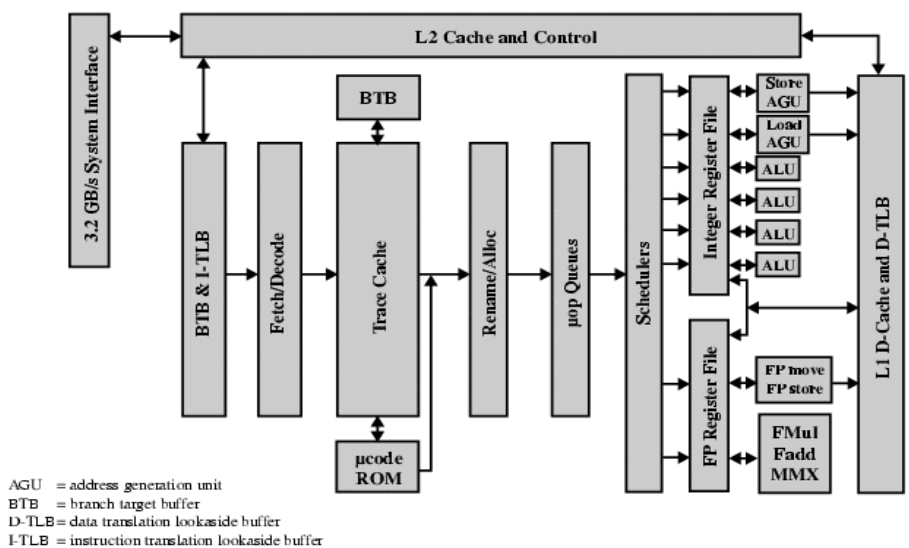
\includegraphics[width=.85\textwidth]{pentium-4}
  \caption{Arquitetura geral do processador do Pentium 4  }
  \label{fig:pentium4}
\end{figure}


\subsection{Very Large Instruction Word - VLIW}
% TODO: indicar se VLIW pode ser conserado RISC ou CISC e porque.

\textsc{Definição} arquitetura que combina diversas operações em uma única instrução muito longa. A tarefa de se determinar quais instruções que serão emitidas simultaneamente, entretanto, recai sobre o compilador.

Neste caso, também teremos diversas unidades funcionais independentes. Uma instrução VLIW poderia incluir 2 operações inteira, 2 de ponto flutuante, 2 referências à memoria e um branch, por exemplo. Dessa forma, se cada unidade funcional tem 16 bits, teríamos um palavra de 112 bits. Note que \textbf{deve haver paralelismo suficiente na sequencia de código para manter todas as unidades ocupadas}.

Como a emissão de instruções e escalonamento é feito pelo compilador, essa arquitetura \textbf{requer pouco ou nenhum \textit{hardware} adicional}. Entretanto, essa abordagem trás alguns problemas:
\begin{itemize}
  \item \textbf{Demandam grande número de portas} sendo uma para cada unidade funcional. Isso aumenta o uso do material - silício - e degrada a velocidade do clock.

  \item Como há múltiplos acessos simultâneos à memória, \textbf{a complexida da memória também aumenta};

  \item \textbf{O tamanho do código aumenta bastante}, apesar de ser possível a implementação de grande quantidade de \textit{loop unrolling};

  \item Quando as instruções não são totalmente cheias, \textbf{temos espaço disperdiçado na VLIW};

  \item Como as operações são emitidas de maneira síncrona, \textbf{um atraso em qualquer unidade funcional, representa um atraso no processador como um todo}
\end{itemize}





\subsection{Análise de Dependência pelo Compilador}
A análise de dependências é fundamental na exploração do paralelismo, uma vez que a detecção destas em um programa é importante para:
\begin{itemize}
  \item Determinar um bom escalonamento de código

  \item \textbf{Determinar os loops que contém paralelismo}, uma vez que essa propriedade existe quando o \textit{loop} não for \textit{loop-carried}. Note que, entre tanto, \textit{loop-carried} não circulares podem ser eliminadas. As verdadeiras limitantes de paralelismo são as dependências \textit{loop-carried} circulares.

  \item Eliminar dependências de nomes
\end{itemize}

Vemos que a determinação da existência de dependências, no caso geral, é um problema NP-Completo. Porém, existem testes exatos para situações restritas que podem ser aplicados, sendo um \textbf{teste considerado exato quando ele determina precisamente que a dependência existe}.

Além de detectar dependências, o compilador deve ser capaz de classificá-las, permitindo que as dependências de nome sejam resolvidas, já que estão identificadas.

Entretanto, em algumas situações, a análise não é efetiva, principalmente uando existem arrays e ponteiros. Temos os casos:
\begin{itemize}
  \item Objetos referenciados via ponteiros;
  \item Indexação indireta de arrays, através de outro array;
  \item Dependência que existe somente em relação a alguns valores de input.
\end{itemize}

	\chapter{Multiprocessadores Simétricos}

\section{Classificação de Arquiteturas}

A divisão das arquiteturas de Flynn possui quatro categorias, segundo o numero de instruções executadas e dados acessados em um instante. Esta divisão foi o primeiro passo na classificação de arquiteturas paralelas e distribuídas. É considerada imprecisa. A Figura \ref{figs:arch-procs} dá a visão geral de todas.

\begin{figure}
  \centering
  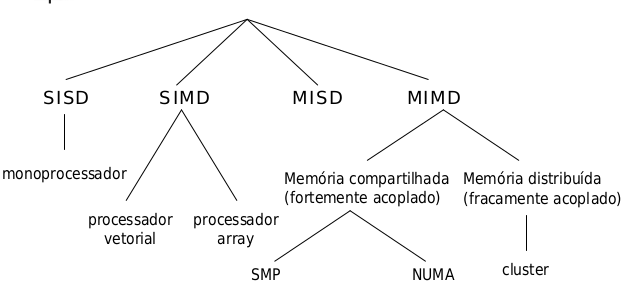
\includegraphics[width=0.9\textwidth]{archs-tree}
  \caption{Taxonomia das Arquiteturas, por Stallings}
  \label{fig:archs-tree}
\end{figure}

\subsubsection{Single Instruction, Single Data (SISD)}
Processadores pipeline e monoprocessadores se encaixam aqui. Possuem os seguintes componentes:

\begin{itemize}
  \item UC: unidade de controle
  \item UP: unidade de processamento, por exemplo a ULA
  \item MEM: memória
\end{itemize}

\subsubsection{Single Instruction, Multiple Data (SIMD)}
A extensão do SISD com multiplicação dos \textit{hardwares} de unidade de processamento e memória (processadores vetoriais). Uma única instrução é buscada e é posta em todos os processadores para execução em posições de memória diferentes. Esta arquitetura é muito usada em GPUs.

\subsubsection{Multiple Instruction, Single Data}
Busca de várias instruções para execução sob um mesmo dado em memória. Dessa forma a replicação está nas unidades de controle e processamento. Esta arquitetura não possui exemplo de caso real, por não fazer sentido.

\subsubsection{Multiple Instruction, Multiple Data (MIMD)}
É uma arquitetura equivalente a multiprocessadores (ou multicores). Além disso, redes de computadores também se encaixam neste exemplo, dado que as unidades representadas são abstratas. Possuem duas arquiteturas:

\begin{itemize}
  \item Fortemente acopladas: Todos os processadores tem acesso direto à memória, sendo ela \textbf{compartilhada}. Exemplo: multiprocessadores;

  \item Fracamente acopladas: cada processadore tem acesso direto apenas a sua memória. Para acesso à outras memórias, \textbf{deve} pedir para o processador detentor da memória alvo. Exemplos: multicomputadores.
\end{itemize}

\begin{figure*}
  \begin{subfigure}{.5\textwidth}
    \centering
    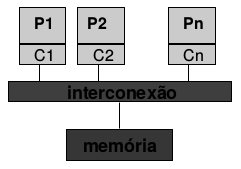
\includegraphics[width=\textwidth, height=4.5cm]{mimd-strong}
    \caption{Fortemente Acoplada}
  \end{subfigure}
  ~
  \begin{subfigure}{.5\textwidth}
    \centering
    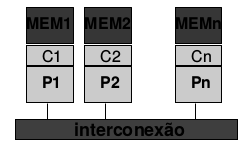
\includegraphics[width=\textwidth]{mimd-weak}
    \caption{Fracamente Acoplada}
  \end{subfigure}

  \caption{Tipos de Arquiteturas MIMD}
\end{figure*}

\begin{figure*}
  \begin{subfigure}{.5\textwidth}
    \centering
    \includegraphics[width=\textwidth]{sisd}
    \caption{SISD}
  \end{subfigure}
  ~
  \begin{subfigure}{.5\textwidth}
    \centering
    \includegraphics[width=\textwidth]{simd}
    \caption{SIMD}
  \end{subfigure}
  ~
  \begin{subfigure}{.5\textwidth}
    \centering
    \includegraphics[width=\textwidth]{misd}
    \caption{MISD}
  \end{subfigure}
  ~
  \begin{subfigure}{.5\textwidth}
    \centering
    \includegraphics[width=\textwidth]{mimd}
    \caption{MIMD}
  \end{subfigure}

  \caption{Tipos de arquiteturas de processadores, segundo Flynn}
  \label{figs:arch-procs}
\end{figure*}




\section{Multiprocessadores Simétricos}

Inicialmente conhecidos como Uniform Memory Access Time (UMA). Possuem dois ou mais processadores com capacidade equivalentes, compartilhando memórias e sistema de I/O, interconectados por um barramento ou crossbar, sendo essa arquitetura \textbf{transparente ao usuário}.

Todos os processadores podem desempenhar as mesmas funções e o sistema é controlado por um sistema operacional integrado. É uma implementação relativamente simples, uma vez que apenas aumentamos o número de processados, mas mantendo mantendo a memória e barramento únicos.

\begin{figure}[ht]
  \centering
  \includegraphics[width=0.6\textwidth]{smp}
  \label{fig:smp}
  \caption{Estrutura de um multiprocessador simétrico. A memória aqui não é necessariamente única}
\end{figure}

\textsc{Definição} \textbf{Crossbar:} vários barramentos de maneira que você consiga uma conexão direta com todos os barramentos, evitando conflito de acesso. Ele é quadrátrico em relação ao número de elementos ($n^2$ conexões quando se tem $n$ elementos). Isso permite a garantia de acesso em tempo uniforme. É um hardware mais caro.

Quando interconectados por barramentos, a arquitetura não é escalável, devido a problemas de contenção no acesso à memória. A cada processador adicionado, existe mais conflito no barramento. Com o crossbar, o problema é o custo do mesmo.

Assim, a introdução cache entre o processador e barramento aliviou um pouco o problema do acesso constante ao barramento, pois o acesso ficou local, gerenciado por algoritmos eficientes de coerência das caches.

Entretanto, mesmo com a introdução da cache, o número de processadores que podem ser conectados ao barramento não chega a 30, sendo geralmente 8. Para tentar resolver o problema de contenção em UMAs, foram propostas arquiteturas NUMA.




\section{Coerência de Cache}
As arquiteturas paralelas fortemente acopladas são afetadas por 3 grandes problemas.

\begin{itemize}
  \item \textbf{Contenção da memória:} ocorre pois cada módulo de memória só pode tratar uma requisição por vez. Logo as requisições para um mesmo módulo são enfileiradas.

  \item \textbf{Contenção de comunicação:} o tempo de latência para redes de interconexão é dado pelo tempo que uma requisição leva para atravessar a rede de interconexão. Isso é diferente de largura de banda, que é a quantidade de informação que pode ser transmitida por uma rede em um determinada tempo.

  \item Tempo de latência
\end{itemize}

As caches em multiprocessadores podem ser:
\begin{itemize}
  \item \textbf{Privadas:} cada processador tem sua cache;
  \item \textbf{Compartilhada:} só existe uma cache, compartilhada entre vários processadores
\end{itemize}

\textsc{Definição} \textbf{Coerência de cache:} garantia que todas as caches possuem sempre o mesmo valor para todas as cópias dos dados, \textbf{quando observadas}.

Logo, queremos garantir que todas as cópias em cache retornem sempre o último valor escrito, ou seja, uma visão coerente e uniforme da memória para todos os processadores, independente do fato de existirem várias caches.

Um \textbf{protocolo de coerência de cache} consistem em:
\begin{itemize}
  \item Um conjunto de estados possíveis das caches locais;
  \item Um conjunto de estados possíveis da memória
  \item Transições de estados causadas por mensagem ou eventos locais.
\end{itemize}




Definimos então duas políticas parada garantir a coerência.

\textsc{Política 1:} \textbf{Write-invalidate}\\
Todas as cópias de um mesmo bloco são invalidadas antes que uma escrita/atualização seja feita em um processador.

Em caso de leitura, se a cópia existir localmente, a operação é feita também localmente. Caso não exista:
\begin{itemize}
  \item Se existir uma cópia em leitura, fazemos uma outra cópia do bloco

  \item Se existir uma cópia em escrita:
  \begin{itemize}
    \item Fazemos uma cópia do bloco e invalidamos a cópia em escrita; ou
    \item Fazemos uma cópia do bloco e tornamos a cópia em escrita um \textit{read-only}
  \end{itemize}
\end{itemize}

\textbf{Premissa:} quando é observada a escrita de um bloco compartilhado, \textbf{invalide} seu bloco.

\underline{Exemplo:} processador $P_1$ quer escrever na sua cache $C_1$ no bloco $b$. Ele avisa aos demais processadores sobre a escrita. Agora, cada processador $P_i$ analisa se ele possui uma cópia de $b$ e caso positivo, ele invalida a cópia. Ao fim, $P_1$ escreve o dado em sua cache. Se $P_i$ desejar obter o bloco invalidado, terá que buscar da memória.\\


\textsc{Política 2:} \textbf{Write-update}\\
As escritas são feitas de maneira atômica em todas cópias dos blocos. Ou seja, assim que uma escrita de um bloco em cache é percebida, a cache solicita o bloco da memória.

\textbf{Premissa:} quando é observada a escrita de um bloco compartilhado, \textbf{atualize} seu bloco.

\underline{Exemplo:} processador $P_1$ quer escrever na sua cache $C_1$ no bloco $b$. Ele avisa aos demais processadores sobre a escrita. Agora, cada processador $P_i$ analisa se ele possui uma cópia de $b$ e caso positivo, ele busca a cópia atualizada e a atualiza. Depois, $P_1$ escreve o dado em sua cache e libera o barramento. No fim, todas as caches estão com os dados atualizados.





\section{Snoopy Caches}
Em arquiteturas conectadas por um barramentos, broadcasts são feitos a cada operação de coerência e assim, as caches sempre estão "escutando" a rede para receber os comandos de coerência. Ao receber um comando, checam se possuem o bloco referênciado e, caso afirmativo, aplicam a operação de coerência. \textbf{Uma cache que implementa esse comportamento é uma snoopy cache}.

\begin{figure}
  \centering
  \includegraphics[width=0.8\textwidth]{snoopy-cache}
  \label{fig:snoopy-cache}
  \caption{Funcionamento de uma snoopy cache}
\end{figure}

Diferentemente das caches de monoprocessadores, as snoopy caches possuem as seguintes características:
\begin{itemize}
  \item O controlador da cache é uma máquina de estados finitos que implementa o protocolo de coerência de acordo com o diagrama de transição de estados;

  \item O difretório da cache precisa acrescentar um conjunto de bits para representar os estados;

  \item O controlador do barramento precisa monitorar toda a operação para descobrir se uma ação é ou não necessária.
\end{itemize}




\subsection{Principais Protocolos de Coerência}
Existem dezenas de protocolos para snoopy caches, dado que eles foram os primeiros protocolos a serem propostos, mas veremos os quatro principais.


\subsubsection{Write Once}
O primeiro protocol \textit{write-invalidate} proposto. É um protocol híbrido, que usa a política \textit{write-through} para a primeira escrita e a política \textit{write-back} para as escritas subsequentes.

\begin{figure}[ht]
  \centering
  \includegraphics[width=\textwidth]{write-once}
  \label{fig:writeonce-automata}
  \caption{Diagrama de estados do \textit{Write Once}}
\end{figure}

\textsc{Transições:}
\begin{itemize}
  \item \textbf{Write-hit:} se a cópia estiver \textsc{Dirty} ou \textsc{Reserved}, o write pode ser feito e o estado da cópia muda para dirty. Se o estado for \textsc{Valid}, é gerado um comando de invalidação \texttt{write\_inv} para todas as caches, a memória é atualizada e a cópia é colocada como \textsc{Reserved};

  \item \textbf{Write-miss:} se não há cópia \textsc{Dirty}, é enviado um comando \texttt{read\_inv} para todas as caches, a cópia é atualizada localmente e o seu estado é \textsc{Dirty}. Se há cópia \textsc{Dirty}, a cópia é fornecida pela cache correspondente, que invalida a sua cópia após o fornecimento. A cópia é alterada localmente e seu estado é \textsc{Dirty}.
\end{itemize}




\subsubsection{Firefly}
É um tipo de protocolo \textit{write-update} que foi implementado em estações de trabalho multiprocessada Firefly. A política utilizada entre as caches e a memória é a de \textit{write-through}. Necessita de uma linha especial de barramento para fazer as atualizações, chamada de \textit{shared line}.

\begin{figure}[ht]
  \centering
  \includegraphics[width=\textwidth]{firefly}
  \label{fig:firefly-automata}
  \caption{Diagrama de estados do Firefly}
\end{figure}




\subsubsection{MSI}
\textsc{Estados}\\
\begin{itemize}
  \item \textbf{Modified} ou Dirty: somente um processador possui uma cópia válida do bloco em sua cache. A cópia da memória principal está incoerente.
  \item \textbf{Shared}: o bloco está presente em diversas caches e está coerente com a memória.
  \item \textbf{Inválida}
\end{itemize}

Este protocol segue a política de cache \textbf{write-back} e é do tipo \textbf{write-invalidate}. \textbf{Note que:}
\begin{itemize}
  \item Ao longo do protocol apenas um processador pode estar no estado \textsc{Modified};

  \item O estado \textsc{Modified} só pode coexistir com estados \textsc{Invalid}.
\end{itemize}

\begin{figure}[ht]
  \centering
  \includegraphics[width=\textwidth]{msi}
  \label{fig:msi-automata}
  \caption{Diagrama de estados do MSI}
\end{figure}



\subsubsection{MESI}
Foram propostos para explicitar o estado onde um dado foi lido com a intenção de ser escrito. A inclusão deste terceiro estado diminui o número de transações no barramento para este caso.

Este protocol segue a política de cache \textbf{write-back} e é do tipo \textbf{write-invalidate}.

\begin{figure}[ht]
  \centering
  \includegraphics[width=\textwidth]{mesi}
  \label{fig:mesi-automata}
  \caption{Diagrama de estados do MESI}
\end{figure}


\textsc{Observações}\\
Protocolos \textit{write-invalidate} apresentam problemas quando existe um escritor e vários leitores. Para esta situação, podemos reduzir o número de \textit{read misses} se, no primeiro read miss que ocorrer, uma cópia for enviada a todas as caches que possuem o bloco no estado \textsc{Invalid}.

Protocolos \textit{write-update} tem o problema de que algumas atualizações podem ser aplicadas em cópias que não mais serão lidas. Por isso, alguns protocols adicionam estados que representam o número de vezes que um bloco foi alterado sem que nenhuma leitura fosse gerada. Se este número atingir um certo limite, as cópias são invalidadas.




\subsection{Protocolos Baseados em Diretórios}
Em algumas arquiteturas, não dispomos de barramento, logo um \textit{broadcast} tem um custo muito alto. Ao invés de usarmos o snoopy cache, fazemos um multicast somente para as caches que com certeza terão o bloco.

Aqui, a memória possui uma lista dos blocos em cache: para cada bloco nas caches, temos a localização de todos os nodos que possuem uma cópia. Esta lista pode ser centralizada ou distribuída e é chamada de \textbf{diretório}.

Em cada entrada do diretório, ou seja, para cada bloco, temos todas as caches que possuem o bloco e um \textit{dirty bit}, indicando a permissão de escrita.




\subsubsection{Full-map Directories}
Aqui, todas as caches do sistema podem abrigar simultaneamente qualquer bloco de dados. Cada entrada de diretório possui, no mínimo, $N$ bits, onde $N$ representa o número de processadores no sistema. Este bit representa o estado do bloco na cache do processador: se está presente ou ausente. Como exemplo, podemos checar a Figura \ref{fig:cache-fullmap}

\begin{figure}
  \centering
  \includegraphics[width=0.6\textwidth]{cache-fullmap}
  \caption{Representação de Diretórios Full-map do estado das caches}
  \label{fig:cache-fullmap}
\end{figure}

\textbf{Escrita}: quando um processador quer escrever, sua cache verifica se o seu bloco local tem permissão de escrita. Caso não, a cache faz \textit{write} para a memória. As demais caches que possuem o bloco recebem o sinal do módulo da memória para invalidar o dado e enviam um \texttt{ACK} para a memória, afim de confirmar. Por fim, o módulo atualiza o diretório e envia a permissão escrita a C3.

Perceba que há um \textit{overhead}: o tamanho de cada entrada de diretório é proporcional ao número de processadores do sistema e isso \textbf{não é escalável}. Por isso, vários esquemas alternativos surgiram.




\subsubsection{Limited Directories}
Propostos com o intuito de \textbf{reduzir o tamanho dos diretórios}. Aqui o número de cópias em cache simultâneas para um bloco particular é limitado.

\textsc{Definição} \textbf{Dir$_{i}X$}, onde $i$ é o número de cópias simultâneas e $X$ pode ser NB (\textit{no broadcast}) ou B (\textit{broadcast}).

São similares aos full-map, exceto no caso onde existem mais de $i$ solicitações de leitura simultâneas. Neste caso, podemos tomar duas atitudes:
\begin{itemize}
  \item $\text{Dir}_i\text{NB}$: uma das cópias é invalidada para dar lugar à nova cópia;

  \item $\text{Dir}_i\text{NB}$: caso haja $j$ cópias em leitura e $j > i$, é enviado um \textit{broadcast} na rede para cada operação de coerência.
\end{itemize}

\textbf{Escrita:} quando um processador $P_i$ quer escrever, sua cache $C_i$ verifica se o bloco local em questão está inválido. Caso positivo, solicita uma cópia da memória, a qual pode detectar que já existem cópias em outras caches distintas. A memória escolhe cópia na cache $C_k$ uma para invalidar (se torna \textit{evicted}) e envia o sinal. A cache $C_k$ recebe a invalidação, seta o bloco como inválido e envia uma confirmação \texttt{ACK} para a memória. Por fim, a memória atualiza o diretório, colocando a $C_i$ no lugar de $C_k$ na posição do bloco solicitado e envia a permissão de escrita para $C_i$.




\subsubsection{Diretórios Encadeados}
É um tipo de diretório \textbf{escalável, porém não limita o número de cópias}. A localização das cópias é obtida através de uma cadeia de ponteiros, como mostrado na Figura \ref{fig:cache-chained-dir}.

\begin{figure}[!ht]
  \centering
  \includegraphics[width=0.6\textwidth]{cache-chained-dir}
  \caption{Representação de Diretórios Encadeados}
  \label{fig:cache-chained-dir}
\end{figure}




\subsubsection{Esquemas Baseados em Software}
Para decidir se o dado é "seguro", temos que marcar todos os dados compartilhados que foram lidos e escritos em algum momento. Marcamos eles como \textit{non-cachable}.

Por fim, precisamos decidir em que fases de um programa uma variável \textit{read-write} pode ser classificada como segura. Ao final da fase, é inserida uma primitiva de invalidação.

	\nocite{*}

	% References
	\bibliographystyle{plain} % Plain referencing style
	\bibliography{references} % Use the example bibliography file sample.bib
\end{document}
